\documentclass[12pt,aspectratio=169]{beamer}

% ====================================================
% ====================================================
% USEPACKAGES AND IMPORTS
% ====================================================
% ====================================================

\usepackage[T1]{fontenc}
\usepackage[utf8]{inputenc}
\usepackage[english]{babel}

% tables
\usepackage{tabularx}
\usepackage{colortbl}
\usepackage{multirow}
\usepackage{makecell}

% tikz and colors
\usepackage{tikz}
\usepackage{xcolor}
\usepackage{pgfplots}
\usepackage{pgfplotstable}
\usepackage{tikzsymbols}

\usetikzlibrary{calc}
\usetikzlibrary{trees}
\usetikzlibrary{patterns}
\usetikzlibrary{shadings}
\usetikzlibrary{positioning}
\usetikzlibrary{intersections}
\usepgfplotslibrary{patchplots}
\usepgfplotslibrary{fillbetween}
\usetikzlibrary{decorations.pathreplacing}

\usetikzlibrary{arrows}
\usetikzlibrary{arrows.meta}

\usetikzlibrary{shapes}
\usetikzlibrary{shapes.arrows}
\usetikzlibrary{shapes.callouts}
\usetikzlibrary{shapes.symbols}
\usetikzlibrary{shapes.geometric}

% boxes
\usepackage[many]{tcolorbox}

% math packages and fonts
\usepackage{bm}
\usepackage{ccfonts}
\usepackage{eulervm}
\usepackage{amsmath}
\usepackage{amsfonts}
\usepackage{amssymb}
\usepackage{amsthm}
\usepackage{mathtools}
\usepackage{nicefrac}
\usepackage{slashed}
\usepackage{bbold}
\usepackage{array}
\usepackage{cancel}

% algorithms and listings
\usepackage[ruled,vlined,linesnumbered]{algorithm2e}
\usepackage{listings}
\usepackage{setspace}

\tcbuselibrary{listings}
\tcbuselibrary{breakable}
\tcbuselibrary{skins}

% misc
\usepackage{soul}
\usepackage{pifont}
\usepackage{skull}
\usepackage{multicol}
\usepackage{animate}
\usepackage{hyperref}
\usepackage{wasysym}
\usepackage[absolute,overlay]{textpos}
\usepackage[hang,flushmargin]{footmisc}

% ====================================================
% ====================================================
% LAYOUT AND THEME
% ====================================================
% ====================================================

\usetheme{Copenhagen}

% color definitions
\definecolor{myblue1}{RGB}{35,119,189}
\definecolor{myblue2}{RGB}{95,179,238}
\definecolor{myblue3}{RGB}{129,168,207}
\definecolor{myblue4}{RGB}{26,89,142}

\definecolor{myred1}{RGB}{247,12,12}

% set theme colors
\setbeamercolor*{structure}{fg=myblue1,bg=blue}
\setbeamercolor*{palette primary}{use=structure,fg=white,bg=structure.fg}
\setbeamercolor*{palette secondary}{use=structure,fg=white,bg=structure.fg!75!black}
\setbeamercolor*{palette tertiary}{use=structure,fg=white,bg=structure.fg!50!black}
\setbeamercolor*{palette quaternary}{fg=black,bg=white}

\setbeamertemplate{itemize item}[circle]
\setbeamertemplate{itemize subitem}[circle]
\setbeamertemplate{itemize subsubitem}[circle]

\setbeamertemplate{enumerate item}[circle]
\setbeamertemplate{enumerate subitem}[circle]
\setbeamertemplate{enumerate subsubitem}[circle]

\setbeamercolor{itemize item}{fg=myblue1}
\setbeamercolor{itemize subitem}{fg=myblue1}
\setbeamercolor{itemize subsubitem}{fg=myblue1}

\setbeamertemplate{section in toc}[circle]
\setbeamertemplate{subsection in toc}[circle]
\setbeamerfont{subsection in toc}{size=\scriptsize}

\setbeamercolor{frametitle continuation}{fg=black}

% title graphic -- sap logo and dhbw logo
\titlegraphic{
\includegraphics[scale=0.1]{../03_img/logo_sap}\hspace*{4.75cm}~%
   	
\includegraphics[scale=0.05]{../03_img/logo_dhbw}
}

\makeatletter
% frame title
\defbeamertemplate*{frametitle}{mydefault}[1][left]
{
  	\ifbeamercolorempty[bg]{frametitle}{}{\nointerlineskip}%
  	\nointerlineskip%
 	\@tempdima=\textwidth%
  	\advance\@tempdima by\beamer@leftmargin%
  	\advance\@tempdima by\beamer@rightmargin%
  	\begin{tcolorbox}[
  		enhanced,
  		outer arc=0pt,
  		arc=0pt,
  		boxrule=0pt,
  		top=0pt,
  		bottom=0pt,
  		enlarge left by=-\beamer@leftmargin,
  		enlarge right by=-\beamer@rightmargin,
  		width=\paperwidth,
  		nobeforeafter,
  		interior style={
    			left color=myblue2,
    			right color=white
    		},
  		shadow={0mm}{-0.4mm}{0mm}{black!60,opacity=0.6},    
  		shadow={0mm}{-0.8mm}{0mm}{black!40,opacity=0.4},    
  	]
    	\usebeamerfont{frametitle}%
    	\vbox{}\vskip-1ex%
    	\if@tempswa\else\csname beamer@fte#1\endcsname\fi%
    	\insertframetitle\par%
    	{%
      		\ifx\insertframesubtitle\@empty%
      		\else%
      		{\usebeamerfont{framesubtitle}\usebeamercolor[fg]{black}\insertframesubtitle\strut\par}%
      		\fi
    	}%
    	\vskip-1ex%
    	\if@tempswa\else\vskip-.3cm\fi
  	\end{tcolorbox}%
}

% footline of a frame
\defbeamertemplate*{footline}{mysplit theme}
{%
  	\leavevmode%
  	\hbox{
		\begin{beamercolorbox}[
			wd=.5\paperwidth,ht=2.5ex,dp=1.125ex,leftskip=.3cm plus1fill,rightskip=.3cm
		]{author in head/foot}%
    			\usebeamerfont{author in head/foot}\insertshortauthor\ (\insertinstitute), \insertdate
  		\end{beamercolorbox}%
  		\begin{beamercolorbox}[
			wd=.5\paperwidth,ht=2.5ex,dp=1.125ex,leftskip=.3cm,rightskip=.3cm plus1fil
		]{title in head/foot}%
    			\usebeamerfont{title in head/foot}\insertshorttitle\hfill
    			\insertprefix-\insertframenumber/\inserttotalframenumber\hspace*{0.5em}
  		\end{beamercolorbox}}%
  	\vskip0pt%
}
\makeatother

% ====================================================
% ====================================================
% COMMANDS AND GENERAL DEFINITIONS
% ====================================================
% ====================================================

% page number prefix
\newcommand\insertprefix{}  % empty by default
\newcommand\prefix[1]{\renewcommand\insertprefix{#1}}

% math definitions
% ====================================================
\DeclareMathOperator*{\argmax}{arg\,max}
\DeclareMathOperator*{\argmin}{arg\,min}
\newcommand*\diff{\mathop{}\!\mathrm{d}}

\newcommand*{\vertbar}{\rule[-1ex]{0.5pt}{2.5ex}}
\newcommand*{\horzbar}{\rule[.5ex]{2.5ex}{0.5pt}}

% commands
% ====================================================

% highlight commands
% --------------------------------------------------------------------------------------------------------
% highlight command
\newcommand{\highlight}[1]{\textcolor{myblue1}{\textbf{#1}}}
\newcommand{\highlighttt}[1]{\textcolor{myblue1}{\texttt{#1}}}
\newcommand{\Highlight}[1]{\textcolor{myred1}{\textbf{#1}}}

% blue color boxes (with frame/without frame/without fill)
\newtcolorbox{boxBlue}{colback=myblue1!10!white,colframe=myblue4}
\newtcolorbox{boxBlueNoFrame}{colback=myblue1!10!white,colframe=myblue1!10!white}
\newtcolorbox{boxBlueNoFill}{colback=white,colframe=myblue4}

% font commands
% --------------------------------------------------------------------------------------------------------
\newcommand{\linkstyle}[1]{\underline{\smash{\texttt{#1}}}} 		% style of hyperlinks

% tikz commands
% --------------------------------------------------------------------------------------------------------

% yellow sticky note
\newcommand{\bubble}[3]{
\begin{textblock}{100}(#1, #2)
      	\begin{tikzpicture}
		\node[rectangle,draw=yellow,very thick,fill=yellow!60,align=center] at (0,0) {#3};
	\end{tikzpicture}
\end{textblock}
}

\newcommand{\floattext}[3]{
\begin{textblock}{100}(#1, #2)
      	#3
\end{textblock}
}

\newcommand{\doublecircle}[2]{
	\draw[fill=white,draw=myblue1] (#1,#2) circle (2mm);
	\draw[fill=myblue1,draw=myblue1] (#1,#2) circle (1.5mm);
}

% slide modifiers
% --------------------------------------------------------------------------------------------------------
% mark slide as optional
\newcommand{\optional}{
	\begin{textblock}{100}(0.15,0.30)
      		
\includegraphics[scale=0.2]{../03_img/scream}
    	\end{textblock}
}

% mark slide as important
\newcommand{\important}{
	\begin{textblock}{100}(0.10,0.15)
      		
\includegraphics[scale=0.1]{../03_img/important}
    	\end{textblock}
}

% citation
% --------------------------------------------------------------------------------------------------------
% first argument in {book, online, article}
\newcommand{\literature}[5]{
	\setbeamertemplate{bibliography item}[#1]
	\bibitem{#2}
	\highlight{#3} \\
	\textcolor{darkgray}{\textit{#4}} \\
	\textcolor{black}{#5}
}
% cite content
\newcommand{\citeAuthor}[3]{\vfill\scriptsize\textcolor{lightgray}{#1 \cite{#2} #3}}

% slide architecture
% --------------------------------------------------------------------------------------------------------
% divide frame into two parts
\newcommand{\divideTwo}[4]{
	\begin{minipage}{#1\textwidth}
		#2
	\end{minipage}
	\hfill
	\begin{minipage}{#3\textwidth}
		#4
	\end{minipage}
}

% divide frame into two parts (start on top)
\newcommand{\divideTwoTop}[4]{
	\begin{minipage}[t]{#1\textwidth}
		#2
	\end{minipage}
	\hfill
	\begin{minipage}[t]{#3\textwidth}
		#4
	\end{minipage}
}

% special pages
% --------------------------------------------------------------------------------------------------------
% title page
\newcommand{\maketitlepage}{
	{
		\beamertemplatenavigationsymbolsempty
		\usebackgroundtemplate{%
			\tikz[overlay,remember picture] \node[opacity=0.2, at=(current page.center)] {
  				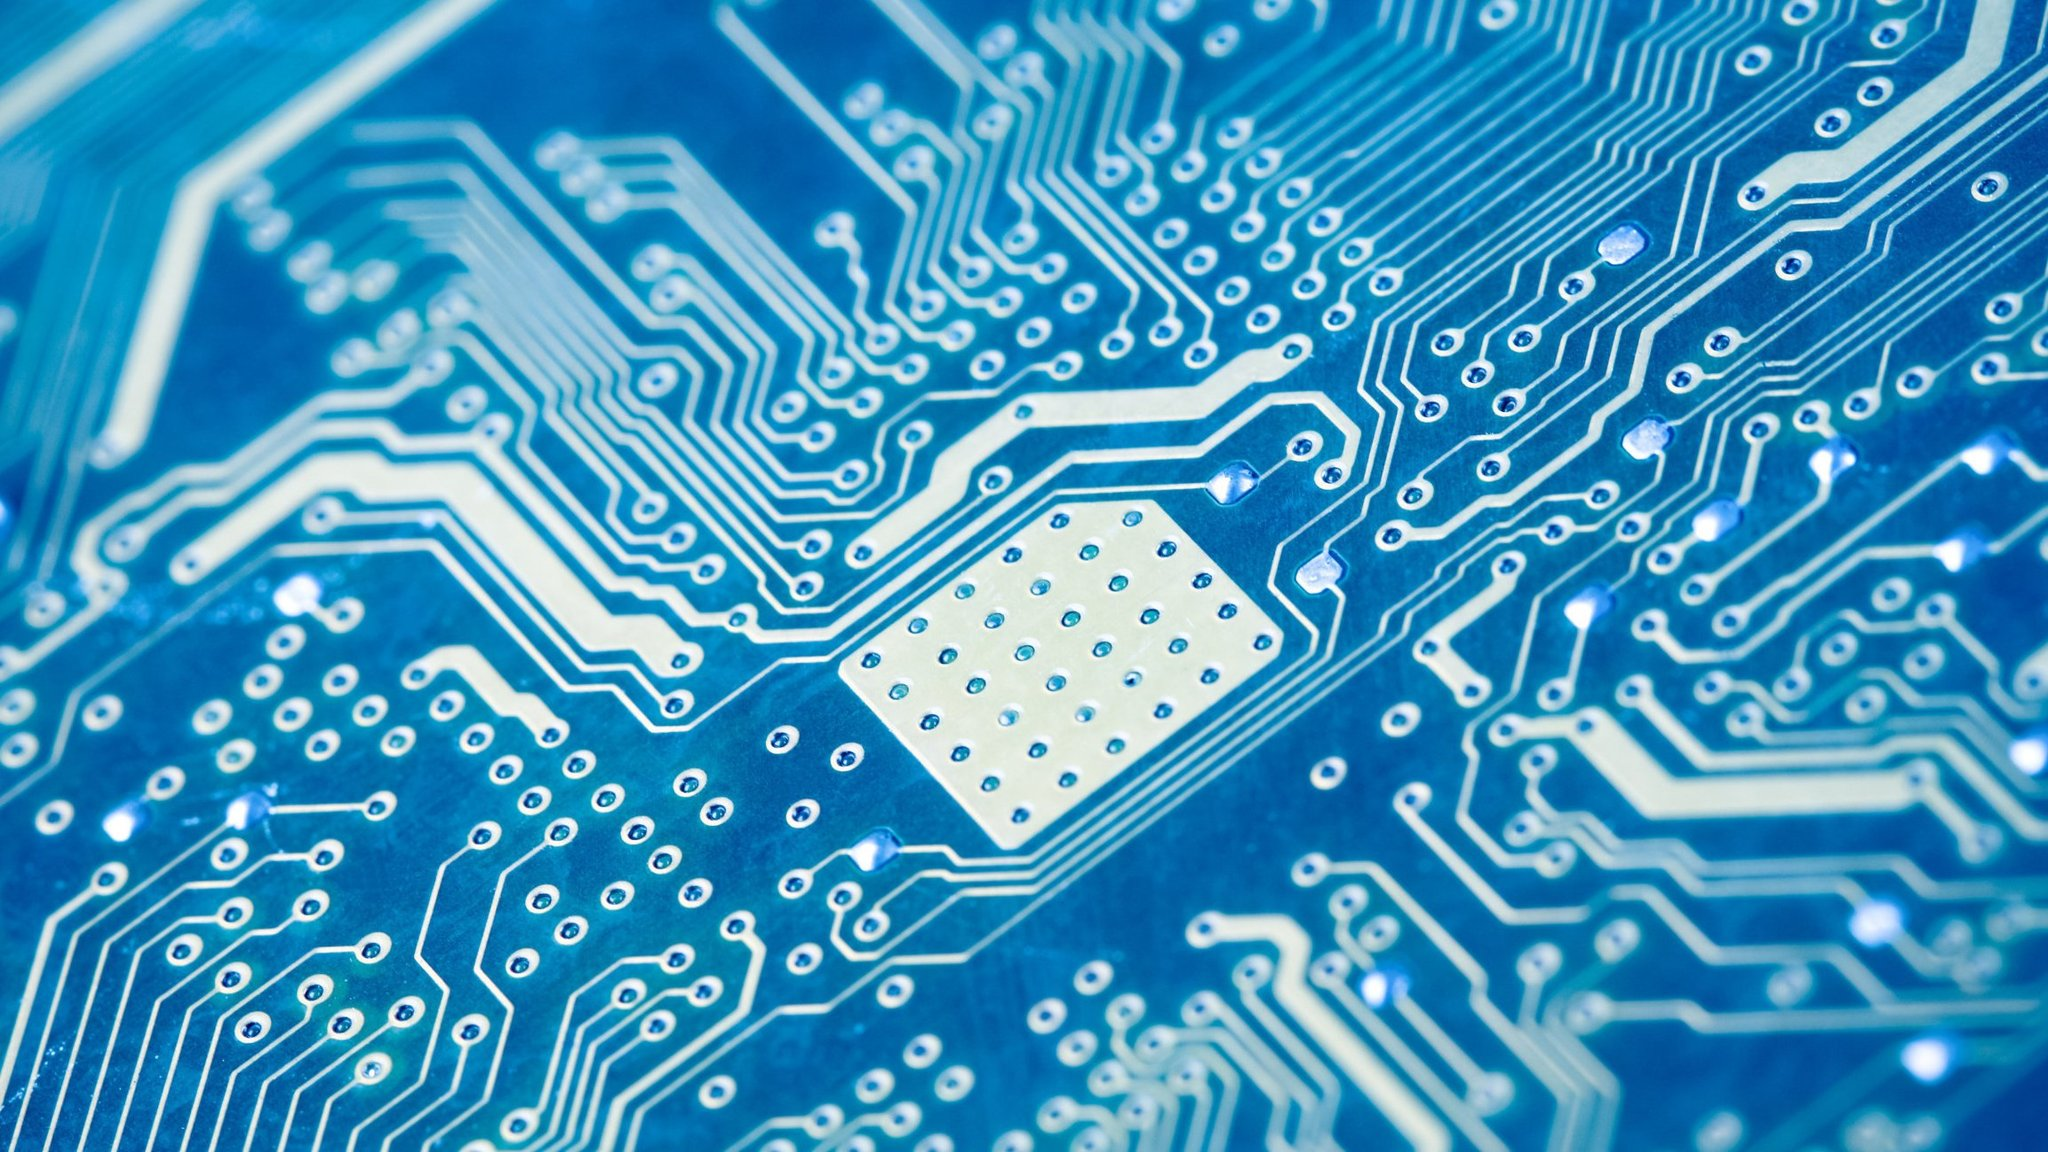
\includegraphics[height=\paperheight,width=\paperwidth]{../03_img/processor.jpg}
			};
		}
		\begin{frame}[plain]
			\vspace*{0.75cm}
			\maketitle
			\vfill
			\begin{center}
				\footnotesize Find all slides on \href{https://github.com/DaWe1992/Applied_ML_Fundamentals}{\linkstyle{GitHub}}
			\end{center}
		\end{frame}
	}
}

% divider page
\newcommand{\makedivider}[1]{
	{
		\beamertemplatenavigationsymbolsempty
		\usebackgroundtemplate{%
			\tikz[overlay,remember picture] \node[opacity=0.2, at=(current page.center)] {
  				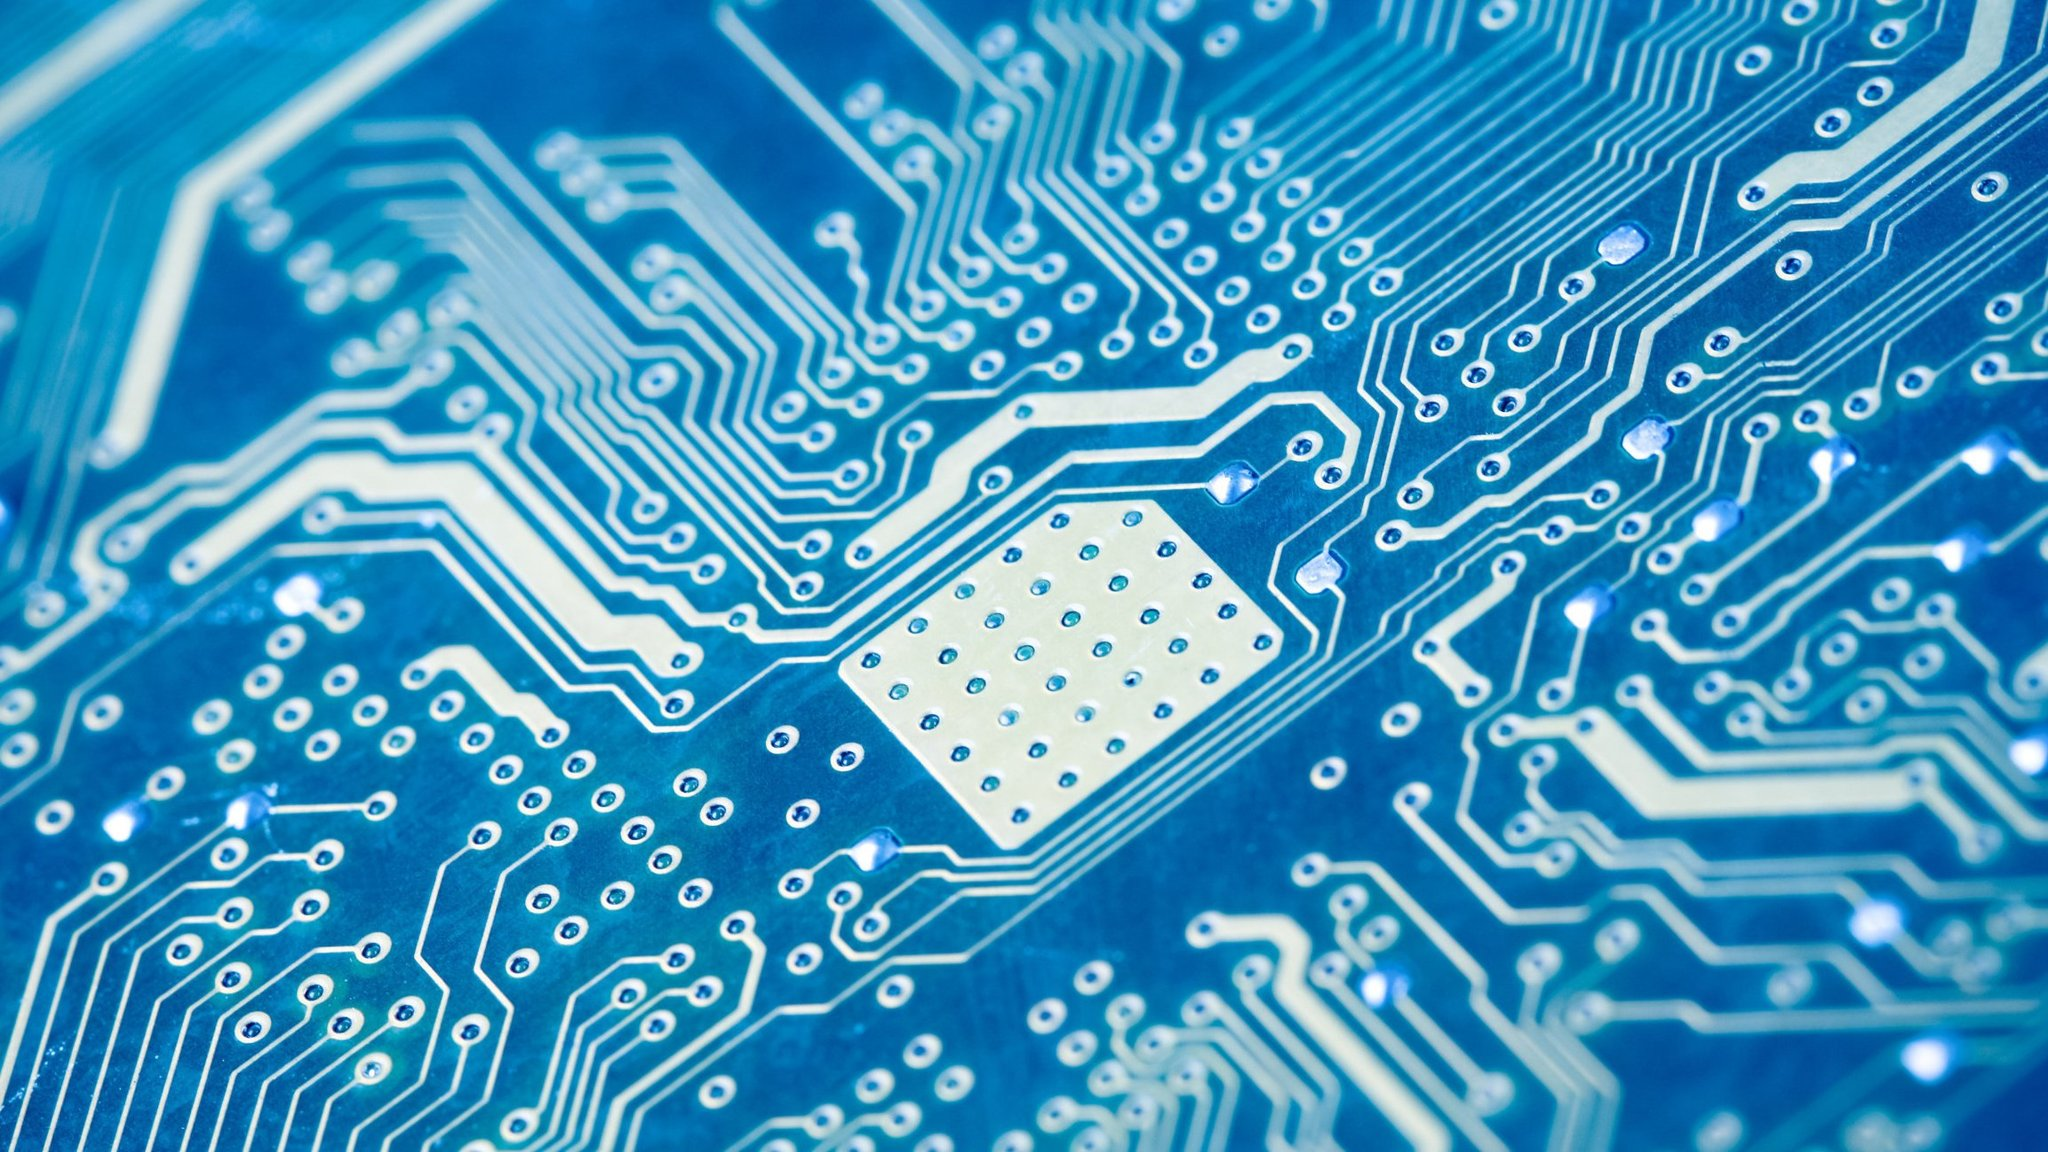
\includegraphics[height=\paperheight,width=\paperwidth]{../03_img/processor.jpg}
			};
		}
		\begin{frame}[plain]
			\vfill
			\begin{boxBlue}
				\centering
				\textbf{Section:} \\
				\large \highlight{#1}
			\end{boxBlue}
			\vfill
			\centering
			
\includegraphics[scale=0.05]{../03_img/logo_dhbw.png}
			\vfill
		\end{frame}
	}
}

% overview page
\newcommand{\makeoverview}[1]{
	\begin{frame}{Lecture Overview}{}
		\begin{tabbing}
			\hspace*{3.5cm}\= \kill
			\ifnum #1=1 \highlight{\textbf{Unit I:}} \else \textbf{Unit I:} \fi
			\> \ifnum #1=1 \highlight{Machine Learning Introduction} \else Machine Learning Introduction \fi \\
		\end{tabbing}
	\end{frame}
}

% thank you page
\newcommand{\makethanks}{
	{\beamertemplatenavigationsymbolsempty
	\begin{frame}[plain]
		\vfill
		\begin{boxBlue}
			\centering
			\Large \highlight{Thank you very much for the attention!}
		\end{boxBlue}
		
		\vfill\footnotesize
		\begin{tabbing}
			\hspace*{1.5cm}\= \kill
			\highlight{Topic:} 	\> \inserttitle \\
			\highlight{Date:} 	\> \insertdate
		\end{tabbing}
		
		\vfill
		\highlight{Contact:} \\
		\insertauthor\ (D062271) \\
		\insertinstitute \\
		\href{mailto:daniel.wehner@sap.com}{\linkstyle{daniel.wehner@sap.com}}
		
		\vfill\normalsize
		\begin{center}
			\large\highlight{Do you have any questions?}
		\end{center}
		\vfill
	\end{frame}}
}

% global pfgplots settings
% --------------------------------------------------------------------------------------------------------
\pgfplotsset{
	% allow filtering of data for pgfplots
	discard if/.style 2 args={
        		x filter/.code={
            		\edef\tempa{\thisrow{#1}}
            		\edef\tempb{#2}
            		\ifx\tempa\tempb
                		\def\pgfmathresult{inf}
            		\fi
        		}
    	},
    	discard if not/.style 2 args={
        		x filter/.code={
            		\edef\tempa{\thisrow{#1}}
            		\edef\tempb{#2}
            		\ifx\tempa\tempb
            		\else
                		\def\pgfmathresult{inf}
            		\fi
        		}
    	}
}


% ====================================================
% ====================================================
% PRESENTATION DATA
% ====================================================
% ====================================================

\title[Support Vector Machines]{*** Applied Machine Learning Fundamentals *** Support Vector Machines}
\institute[SAP\,SE]{SAP\,SE / DHBW Mannheim}
\author{Daniel Wehner, M.Sc.}
\date{Winter term 2020/2021}
\prefix{SVM}

% ====================================================
% ====================================================
% BEGIN OF DOCUMENT
% ====================================================
% ====================================================

\begin{document}

% Title frame
%______________________________________________________________________
\maketitlepage


% Lecture Overview
%______________________________________________________________________
\begin{frame}{Lecture Overview}{}
	\makeoverview{8}
\end{frame}


% Agenda
%______________________________________________________________________
\begin{frame}{Agenda for this Unit}
	\begin{multicols}{2}
		\tableofcontents
	\end{multicols}
\end{frame}


% Section: Linear SVMs
%______________________________________________________________________
\section{Linear SVMs}
\makedivider{Linear SVMs}

% Subsection: Introduction
% --------------------------------------------------------------------------------------------------------
\subsection{Introduction}

% What is a Support Vector Machine (SVM)?
\begin{frame}{What is a Support Vector Machine (SVM)?}{}
	\begin{itemize}
		\item A support vector machine is a \textbf{binary classifier}
			{\footnotesize [Vapnik and Chervonenkis]}
		\begin{itemize}
			\item The classes are denoted by $\{-1; +1\}$
			\item Techniques for multi-class classification: One-vs-Rest and One-vs-One
		\end{itemize}
		\item The algorithm was introduced in the 60s, extensions were made in the 90s
		\item An SVM finds the \textbf{best separating hyperplane}
		\item \textbf{Question:} \textit{What is the best separating hyperplane?}
		\item Why is it called \textit{`machine'}?
		\begin{itemize}
			\item It's no physical machine, it's a mathematical construct
			\item `Machine' refers to `Machine Learning' 
		\end{itemize}
	\end{itemize}
\end{frame}


% Discriminant Functions
\begin{frame}{Discriminant Functions}{}
	\begin{itemize}
		\item The simplest discriminant is a linear function of the form:
		\begin{equation}
			\widehat{h}(\bm{x})
				= \bm{w}^{\intercal} \bm{x} + b
				= \sum_{j=1}^m w_j x_j + b
				= w_1 x_1 + w_2 x_2 + \dots + w_m x_m + b
		\end{equation} 
		\item $\bm{\theta} = \{ \bm{w}, b \}$: $\bm{w}$ is called the \textbf{weight vector} and $b$ is the \textbf{bias}
		\item An input vector $\bm{x}$ is assigned class $\mathcal{C}_1$, if $\widehat{h}(\bm{x}) \ge 0$,
			class $\mathcal{C}_2$ otherwise
		\item The \highlight{decision boundary} is defined by the relation: $\widehat{h}(\bm{x}) = 0$
		\item The boundary is a $(D - 1)$-dimensional hyperplane within the $D$-dimensional input space
	\end{itemize}
\end{frame}


% Discriminant Functions (Ctd.)
\begin{frame}{Discriminant Functions (Ctd.)}{}
	\vspace*{-2mm}
	\begin{figure}
	\centering
	\begin{tikzpicture}[
		scale=0.7
	]

		\fill[fill=gray,fill opacity=0.3] (-1,4.8) -- (-1,5.5) -- (6.5,5.5) -- (6.5,-0.8) -- (6,-0.8) -- cycle;
		\fill[fill=lightgray,fill opacity=0.2] (-1,4.8) -- (-1,-0.8) -- (6,-0.8) -- cycle;

		\draw[very thick,double,line cap=rect,red] (-1,4.8) -- (6,-0.8);
		\draw[very thick,blue,->] (0,0) -- (6,3) node[right] {$\bm{x}$};
		\draw[thick,dashed,blue] (6,3) -- node[right=2mm] {$\frac{y(\bm{x})}{\Vert \bm{w} \Vert}$} (4.15,0.69)
			node[below] {$\bm{x}_{\perp}$};
		\draw[very thick,green,->] (0,0) -- node[above] {$\bm{w}$} (1,1.25);
		\draw[thick,dashed,green] (1,1.25) -- (1.95,2.44);
		
		\draw (0,0) -- (3,-2.4);
		\draw[<->,thick] (3.5,1.2) -- node[below right=-1mm] {$\frac{-b}{\Vert \bm{w} \Vert}$} (1.55,-1.24);

		% axes
		\draw[thick,->] (0,0) -- (7,0) node[right] {$x_1$};
		\draw[thick,->] (0,0) -- (0,6) node[left] {$x_2$};

		\node at (3,4) {\scriptsize\textbf{Class +1}};
		\node at (0.75,2.5) {\scriptsize\textbf{Class -1}};

	\end{tikzpicture}
\end{figure}
\end{frame}


% Discriminant Functions (Ctd.)
\begin{frame}{Discriminant Functions (Ctd.)}{}
	\begin{itemize}
		\item Consider two points, $\bm{x}_A$ and $\bm{x}_B$, which lie on the decision surface
		\item Since $\widehat{h}(\bm{x}_A) = \widehat{h}(\bm{x}_B) = 0$, we have $\bm{w}^{\intercal}(\bm{x}_A - \bm{x}_B) = 0$,
			hence $\bm{w}$ is \textbf{orthogonal} to every vector lying within the decision surface
		\item $\bm{w}$ determines the orientation of the decision surface
		\item Similarly, if $\bm{x}$ is a point on the decision surface, then $\widehat{h}(\bm{x}) = 0$ and the normal distance from the
			origin to the decision surface is given by:
		\begin{equation}
			\frac{\bm{w}^{\intercal} \bm{x} + b}{\Vert \bm{w} \Vert} = 0
			\Leftrightarrow
			\frac{\bm{w}^{\intercal} \bm{x}}{\Vert \bm{w} \Vert} = -\frac{b}{\Vert \bm{w} \Vert}
		\end{equation}
		\item $b$ controls the offset from the origin
	\end{itemize}
\end{frame}


% Discriminant Functions (Ctd.)
\begin{frame}{Discriminant Functions (Ctd.)}{}
	\begin{itemize}
		\item $\widehat{h}(\bm{x})$ gives a \textbf{signed measure} of the perp. distance of $\bm{x}$ to the boundary
		\item Consider an arbitrary point $\bm{x}$ and its orth. projection $\bm{x}_{\perp}$ onto the surface
		\begin{equation}
			\bm{x} = \bm{x}_{\perp} + r \frac{\bm{w}}{\Vert \bm{w} \Vert}
		\end{equation}
		\item Multiplying both sides by $\bm{w}^{\intercal}$ and adding $b$, and making use of:
		\begin{equation*}
			\widehat{h}(\bm{x})
				= \bm{w}^{\intercal} \bm{x} + b \qquad \text{and} \qquad
			\widehat{h}(\bm{x}_{\perp})
				= \bm{w}^{\intercal} \bm{x}_{\perp} + b = 0			
		\end{equation*}
		\item We get:
		\begin{equation}
			r = \frac{\widehat{h}(\bm{x})}{\Vert \bm{w} \Vert}
		\end{equation}
	\end{itemize}
\end{frame}


% Linear Separability
\begin{frame}{Linear Separability}{}
	\begin{itemize}
		\item We have $n$ input vectors $\bm{X} = \{ \bm{x}^{(1)}, \bm{x}^{(2)}, \dots, \bm{x}^{(n)} \}$
		\item With corresponding target values $y^{(1)}, y^{(2)}, \dots, y^{(n)}$, where $y^{(i)} \in \{-1, +1\}$
		\item New data points are classified according to the sign of $\widehat{h}(\bm{x})$: $sign(\widehat{h}(\bm{x}))$
	\end{itemize}
	
	\vspace*{1mm}
	\begin{boxBlueNoFrame}
		\footnotesize
		A data set is \textbf{linearly separable} in feature space, if $\exists (\bm{w}, b)$ such that
		\begin{align}
			\widehat{h}(\bm{x}^{(i)}) = \bm{w}^{\intercal} \bm{x}^{(i)} + b &> 0 \qquad
				\text{$\forall \bm{x}^{(i)}$ with $y^{(i)} = +1$} \\
			\widehat{h}(\bm{x}^{(i)}) = \bm{w}^{\intercal} \bm{x}^{(i)} + b &< 0 \qquad
				\text{otherwise ($y^{(i)} = -1$)}
		\end{align}
		This can also be written as: $y^{(i)} \widehat{h}(\bm{x}^{(i)}) > 0\ \forall i$ 
	\end{boxBlueNoFrame}
\end{frame}


% Example Data Set
\begin{frame}{Example Data Set (linearly separable)}{}
	\divideTwo{0.49}{
		\vspace*{6mm}
		\begin{figure}
	\centering
	\begin{tikzpicture}[
		scale=0.8
	]

		\begin{axis}[
			xlabel={$x_1$},
			ylabel={$x_2$}
		]
		
			\addplot[
				only marks,mark=*,mark size=2.0,fill=myblue1,discard if not={c}{-1}
			] table{11_svm/05_data/data_linearly_separable.txt};

			\addplot[
				only marks,mark=*,mark size=2.0,fill=lightgray,discard if not={c}{1}
			] table{11_svm/05_data/data_linearly_separable.txt};
    		\end{axis}

	\end{tikzpicture}
\end{figure}
	}{0.49}{
		\vspace*{-2mm}
		\begin{itemize}
			\item This data set is \highlight{linearly separable} (you can find a straight line to separate the two classes)
			\item The possible number of hyperplanes is infinite...
			\item \textbf{Which hyperplane should be chosen?}
		\end{itemize}
	}
\end{frame}


% Subsection: Maximum Margin Classifiers
% --------------------------------------------------------------------------------------------------------
\subsection{Maximum Margin Classifiers}

% Maximum Margin Classifiers
\begin{frame}{Maximum Margin Classifiers}{}\important
	\divideTwo{0.54}{
		\begin{itemize}
			\item An SVM is a so-called \highlight{maximum margin classifier}
			\item It maximizes the margin $\mathcal{M}$
			\begin{equation*}
				\max_{\bm{w}, b} \mathcal{M}
			\end{equation*}
			\item The larger $\mathcal{M}$ the less likely are false predictions
			\item Only the \highlight{support vectors} determine the hyperplane
		\end{itemize}
	}{0.44}{
		\begin{figure}
	\centering
	\begin{tikzpicture}[
		scale=0.8,
		arrow/.style={
			orange,->,
			shorten >=2pt,shorten <=2pt
		},
		class1/.style={
			star,star points=10,
			inner sep=3pt
		},
		class2/.style={
			diamond,
			inner sep=3pt
		}
	]

		\draw[draw=white,fill=myblue3,fill opacity=0.2] (0,0.5) -- (0,0) -- (3,0) -- (6,3) -- (6,6.5) -- cycle;
	
		\draw[gray,dashed,thick] (0,0.5) -- (6,6.5);
		\draw[gray,dashed,thick] (3,0) -- (6,3);
		\draw[very thick,myblue1] (1.25,0) -- (6,4.75);
		\draw[dotted,red,thick,<->] (2,2.5) --
			node[left,rotate=45] {\tiny $\mathcal{M} = \nicefrac{1}{\Vert \bm{w} \Vert}$} (2.875,1.625);

		\node[fill=orange] (A) at (2,6) {\tiny \textbf{Support Vectors} $\bm{\mathcal{S}}$};

		% draw support vectors
		\node[draw=magenta,thick,fill=yellow,class1] (SV1) at (2.5,3) {};
		\node[draw=magenta,thick,fill=yellow,class1] (SV2) at (1.5,2) {};
		\node[draw=cyan,thick,fill=yellow,class2] (SV3) at (4.25,1.25) {};

		\draw[arrow] (A) -- (SV1);
		\draw[arrow] (A) -- (SV2);
		\draw[arrow] (A) -- (SV3);

		% axes
		\draw[thick,->] (0,0) -- (7,0) node[right] {$x_1$};
		\draw[thick,->] (0,0) -- (0,6.5) node[left] {$x_2$};

		\foreach \x/\y in {1/3,2/4,1/4}
			\node[draw=magenta,fill=white,class1] at (\x,\y) {};
		\foreach \x/\y in {6/1.75,4.5/0.75,5.75/1,5.25/0.5,6.5/0.75}
			\node[draw=cyan,fill=white,class2] at (\x,\y) {};

		\node[gray,rotate=45] at (5,5) {\tiny $\bm{w}^{\intercal} \bm{x} + b = +1$};
		\node[gray,rotate=45] at (5,2.5) {\tiny $\bm{w}^{\intercal} \bm{x} + b = -1$};
		\node[myblue1,rotate=45] at (5,3.25) {\tiny $\bm{w}^{\intercal} \bm{x} + b = 0$};

	\end{tikzpicture}
\end{figure}
	}
\end{frame}


% Maximum Margin Classifiers (Ctd.)
\begin{frame}{Maximum Margin Classifiers (Ctd.)}{}
	\begin{itemize}
		\item Recall the perpendicular distance of a point $\bm{x}$ to the hyperplane:
		\begin{equation}
			\frac{\vert \widehat{h}(\bm{x}) \vert}{\Vert \bm{w} \Vert}
		\end{equation}
		\item Furthermore, we are only interested in solutions for which all data points are correctly classified, i.\,e. 
			$y^{(i)} \widehat{h}(\bm{x}^{(i)}) > 0\ \forall i$, thus the distance is given by:
		\begin{equation}
			\frac{y^{(i)} \widehat{h}(\bm{x}^{(i)})}{\Vert \bm{w} \Vert} = \frac{y^{(i)} (\bm{w}^{\intercal} \bm{x}^{(i)} + b)}{\Vert \bm{w} \Vert}
		\end{equation}
	\end{itemize}
\end{frame}


% Maximum Margin Classifiers (Ctd.)
\begin{frame}{Maximum Margin Classifiers (Ctd.)}{}
	\begin{itemize}
		\item The margin is given by the perp. distance to the closest data point $\bm{x}^{(i)}$
		\item We wish to optimize the parameters $\bm{w}$ and $b$ to maximize this distance
		\item We have to solve:
		\vspace*{-3.5mm}
		\begin{equation}
			\bm{w}^*, b^* =
			\overbracket{
				\argmax_{\bm{w}, b} \left\{ \frac{1}{\Vert \bm{w} \Vert}
				\overbracket{
					\min_i \{y^{(i)} (\bm{w}^{\intercal} \bm{x}^{(i)} + b)\}
				}^{\text{`closest data points'}}
				\right\}
			}^{\text{`maximize distance to closest data points'}}
		\end{equation}
		\vspace*{-3.5mm}
		\item Note that $1/\Vert \bm{w} \Vert$ does not depend on $i$
		\item A direct solution of this optimization would be very complex $\Rightarrow$ rewrite!
	\end{itemize}
\end{frame}


% Maximum Margin Classifiers (Ctd.)
\begin{frame}{Maximum Margin Classifiers (Ctd.)}{}
	\begin{itemize}
		\item We note that rescaling $\bm{w}$ and $b$ by a factor $\zeta$
			\textbf{does not change the distance} to the decision boundary
		\item Therefore, for the points that are closest to the surface, we can set:
		\begin{equation}
			y^{(i)} (\bm{w}^{\intercal} \bm{x}^{(i)} + b) = 1
		\end{equation}
		\item In this case, all data points $\bm{x}^{(i)}$ satisfy the constraint:
		\begin{equation}
			y^{(i)} (\bm{w}^{\intercal} \bm{x}^{(i)} + b) \ge 1 \qquad i = 1, 2, \dots, n
		\end{equation}
		\item It is sufficient to solve: \highlight{$\argmin_{\bm{w}, b} \frac{1}{2} \Vert \bm{w} \Vert^2$}
			\footnotesize ($\nicefrac{1}{2}$ for mathematical convenience) \normalsize
	\end{itemize}
\end{frame}


% Maximum Margin Classifiers (Ctd.)
\begin{frame}{Maximum Margin Classifiers (Ctd.)}{}
	\vspace*{-4mm}
	\begin{equation}
		\bm{w}^*, b^* = \argmin_{\bm{w}, b} \frac{1}{2} \Vert \bm{w} \Vert^2
	\end{equation}
	\vspace*{4mm}
	
	\divideTwo{0.75}{
		\begin{itemize}
			\item This is a \textbf{quadratic optimization (QP)} problem
			\item A global optimum exists due to \textbf{convexity}
			\item How to solve such problems?
		\end{itemize}
		\vspace*{2mm}\centering
		\highlight{Lagrangian optimization} \\
		\footnotesize (named after Joseph-Louis Lagrange)
	}{0.24}{
		\vspace*{2mm}
		\begin{figure}
			\centering
			\fbox{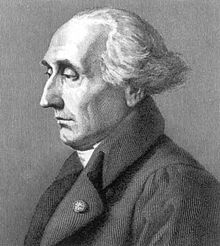
\includegraphics[scale=0.3]{11_svm/02_img/lagrange}}
		\end{figure}
	}
\end{frame}


% Subsection: Lagrangian Optimization
% --------------------------------------------------------------------------------------------------------
\subsection{Lagrangian Optimization}

% Lagrangian Optimization: A simple Example
\begin{frame}{Lagrangian Optimization: A simple Example}{}
	\begin{itemize}
		\item Lagrangian optimization is optimization \textbf{subject to constraints}
		\item \textbf{Example:}
		\begin{equation}
			\overbracket{f(x_1, x_2) = 1 - x_1^2 - x_2^2}^{\text{function to optimize $f(\bm{x})$}}
			\quad \text{s.\,t.} \quad
			\overbracket{g(x_1, x_2) = x_1 + x_2 - 1 = 0}^{\text{linear constraint $g(\bm{x}) = 0$}}
		\end{equation}
		\item To find a solution we have to formulate the \highlight{Lagrangian equation}: \\
			{\footnotesize General form: $\mathcal{L}(\bm{x}, \alpha) = f(\bm{x}) + \alpha g(\bm{x})$}
		\begin{equation}
			\mathcal{L}(\bm{x}, \alpha) = 1 - x_1^2 - x_2^2 + \alpha(x_1 + x_2 - 1)
		\end{equation}
	\end{itemize}
\end{frame}


% Lagrangian Optimization: A simple Example (Ctd.)
\begin{frame}{Lagrangian Optimization: A simple Example (Ctd.)}{}
	\begin{equation*}
		\mathcal{L}(\bm{x}, \alpha) = 1 - x_1^2 - x_2^2 + \alpha(x_1 + x_2 - 1)
	\end{equation*}
	
	We determine the partial derivatives w.\,r.\,t. $x_1$, $x_2$ and $\alpha$ and set them to zero:
	\begin{alignat}{2}
		\frac{\partial \mathcal{L}(\bm{x}, \alpha)}{\partial x_1} 	&= -2 x_1 + \alpha	&&\overset{!}{=} 0 	\\[2mm]
		\frac{\partial \mathcal{L}(\bm{x}, \alpha)}{\partial x_2} 	&= -2 x_2 + \alpha 	&&\overset{!}{=} 0	\\[2mm]
		\frac{\partial \mathcal{L}(\bm{x}, \alpha)}{\partial \alpha} 	&= x_1 + x_2 - 1 	&&\overset{!}{=} 0
	\end{alignat}
\end{frame}


% Lagrangian Optimization: A simple Example (Ctd.)
\begin{frame}{Lagrangian Optimization: A simple Example (Ctd.)}{}
	\begin{itemize}
		\item Solving the first two equations for $x_1$ and $x_2$, respectively, we get:
		\begin{align}
			x_1 &= \nicefrac{1}{2} \alpha \\
			x_2 &= \nicefrac{1}{2} \alpha
		\end{align}
		\item Substitution into the third equation $x_1 + x_2 - 1 = 0$:
		\begin{equation}
			\widetilde{\mathcal{L}}(\alpha) =
				\nicefrac{1}{2} \alpha + \nicefrac{1}{2} \alpha - 1 = 0 \Leftrightarrow \alpha = 1
		\end{equation}
		\item Finally, we get:
		\begin{equation*}
			x_1 = \nicefrac{1}{2} \qquad x_2 = \nicefrac{1}{2}
		\end{equation*}
	\end{itemize}
\end{frame}


% Lagrangian Optimization: A simple Example (Ctd.)
\begin{frame}{Lagrangian Optimization: A simple Example (Ctd.)}{}
	\begin{figure}
	\centering
	\begin{tikzpicture}[
		scale=0.8
	]

		\begin{axis}[
			legend pos=outer north east,
			xlabel={$x_1$},
    			ylabel={$x_2$},
    			zlabel={$y$}
		]

			\addplot3[
				surf,
				colormap/hot2,
				samples=41
			] {1-x^2-y^2};

			\addplot3[
				ultra thick,
				samples y=1,
				blue!70,
				smooth
			] table[z expr=1-x^2-y^2]
    			{
        			x  y
				5 -4
				4  -3
				3  -2
				2  -1
				1  0
				0  1
				-1  2
    			};
    				
			\addplot3[
				scatter,
				only marks,
				red
			] table[z expr=1-x^2-y^2]
			{
				x  y
				0.5  0.5
			};

			\addplot3[
				scatter,
				only marks,
				mark=oplus,
				red!80!black
			] table[z expr=1-x^2-y^2]
			{
				x  y
				0  0
			};

			\legend{$f(\bm{x})$, $g(\bm{x}) = 0$, Constrained optimum, Global optimum}
		\end{axis}
		
	\end{tikzpicture}
\end{figure}
\end{frame}


% SVM Parameter Optimization
\begin{frame}{SVM Parameter Optimization}{}
	\begin{boxBlueNoFrame}
		We have to solve the Lagrangian:
		\begin{equation}
			\mathcal{L}(\bm{w}, b, \bm{\alpha}) = \overbracket{
				\nicefrac{1}{2} \Vert \bm{w} \Vert^2
			}^{f(\bm{x})} -
			\sum_{i=1}^n \alpha_i [\overbracket{
				y^{(i)} \cdot (\bm{w}^{\intercal} \bm{x}^{(i)} + b) - 1
			}^{g(\bm{x})\, =\, 0}]
		\end{equation}
	\end{boxBlueNoFrame}
	\begin{itemize}
		\item $\bm{\alpha}$ is a vector of \highlight{Lagrangian multipliers}
		\item There is \textbf{one constraint per data point!}
		\item The Lagrangian multipliers will be non-zero for all support vectors
	\end{itemize}
\end{frame}


% SVM Parameter Optimization (Ctd.)
\begin{frame}{SVM Parameter Optimization (Ctd.)}{}\important
	\floattext{8.75}{6.25}{\footnotesize \highlight{linear combination of input!}}
	We have to compute the partial derivatives w.\,r.\,t. $\bm{w}$ and b and set them to zero:
		
	\begin{alignat}{2}
		\frac{\partial \mathcal{L}}{\partial \bm{w}}
			&= \bm{w} - \sum_{i=1}^n \alpha_i y^{(i)} \bm{x}^{(i)} \overset{!}{=} 0
				&&\Rightarrow \boxed{\bm{w} = \sum_{i=1}^n \alpha_i y^{(i)} \bm{x}^{(i)}} \\[5mm]
		\frac{\partial \mathcal{L}}{\partial b} 
			&= -\sum_{i=1}^n \alpha_i y^{(i)} \overset{!}{=} 0
				&&\Rightarrow \boxed{\sum_{i=1}^n \alpha_i y^{(i)} = 0}
	\end{alignat}
\end{frame}


% SVM Parameter Optimization (Ctd.)
\begin{frame}{SVM Parameter Optimization (Ctd.)}{}\optional
	\floattext{4.75}{14}{\footnotesize \highlight{Wolfe dual}}
	As a next step the partial derivatives are substituted in into $\mathcal{L}$:
	\footnotesize
	\begin{align}
		\nonumber
		\widetilde{\mathcal{L}}(\bm{\alpha})
		&=
			\frac{1}{2} \left( \sum_{i=1}^n \alpha_i y^{(i)} \bm{x}^{(i)} \right)\left( \sum_{j=1}^n \alpha_j y^{(j)} \bm{x}^{(j)} \right) -
			\left( \sum_{i=1}^n \alpha_i y^{(i)} \bm{x}^{(i)} \right) \left( \sum_{j=1}^n \alpha_j y^{(j)} \bm{x}^{(j)} \right) \\
		&\phantom{=} - \sum_{i=1}^n \alpha_i y^{(i)} b + \sum_{i=1}^n \alpha_i \\[5mm]
		&=
			\boxed{
				\sum_{i=1}^n \alpha_i - \frac{1}{2} \sum_{i=1}^n \sum_{j=1}^n
					\alpha_i \alpha_j y^{(i)} y^{(j)} \langle \bm{x}^{(i)}, \bm{x}^{(j)} \rangle
			} \quad \text{s.\,t.}\ \alpha_i \ge 0\ \forall i\ \text{and}\ \sum_{i=1}^n \alpha_i y^{(i)} = 0
	\end{align}
	\normalsize
\end{frame}


% SVM Parameter Optimization (Ctd.)
\begin{frame}{SVM Parameter Optimization (Ctd.)}{}\optional
	\begin{itemize}
		\item Once we know $\bm{\alpha}$, we can determine $b$ by noting that any
			support vector satisfies $y^{(i)} \widehat{h}(\bm{x}^{(i)}) = 1$: {\scriptsize ($\mathcal{S} \equiv$ indices of support vectors)}
		\begin{equation}
			y^{(i)} \left( \sum_{j \in \mathcal{S}} \alpha_j y^{(j)} \langle \bm{x}^{(i)}, \bm{x}^{(j)} \rangle + b \right) = 1
		\end{equation}
		\item Average over all support vectors to compute $b$: {\scriptsize ($n_\mathcal{S} \equiv$ number of support vectors)}
		\begin{equation}
			b = \frac{1}{n_{\mathcal{S}}} \sum_{i \in \mathcal{S}} \left(
				y^{(i)} - \sum_{j \in \mathcal{S}} \alpha_j y^{(j)} \langle \bm{x}^{(i)}, \bm{x}^{(j)} \rangle
			\right)
		\end{equation}
	\end{itemize}
\end{frame}


% Updated Decision Rule
\begin{frame}{Updated Decision Rule}{}
	\begin{itemize}
		\item Given our derivations, we can rewrite the SVM decision rule as follows:
		\begin{equation}
			h(\bm{x}) = sign\left( \sum_{i \in \mathcal{S}} \alpha_i y^{(i)} \langle \bm{x}^{(i)}, \bm{x} \rangle + b \right)
		\end{equation}
		\item $\bm{x}$ is an unknown instance for which the class label is not known
	\end{itemize}

	\vspace*{2mm}
	\begin{boxBlueNoFrame}
		\footnotesize
		\highlight{Since all $\alpha_i$ will be zero for non-support vectors, the decision
		for a class depends on the support vectors only!} This makes predictions fast, even for large data sets.
		\textbf{The number of support vectors can also be used as an evaluation criterion.}
	\end{boxBlueNoFrame}
\end{frame}


% Linear SVM: Example
\begin{frame}{Linear SVM: Example}{}
	\vspace*{-2mm}
	\begin{figure}
		\centering
		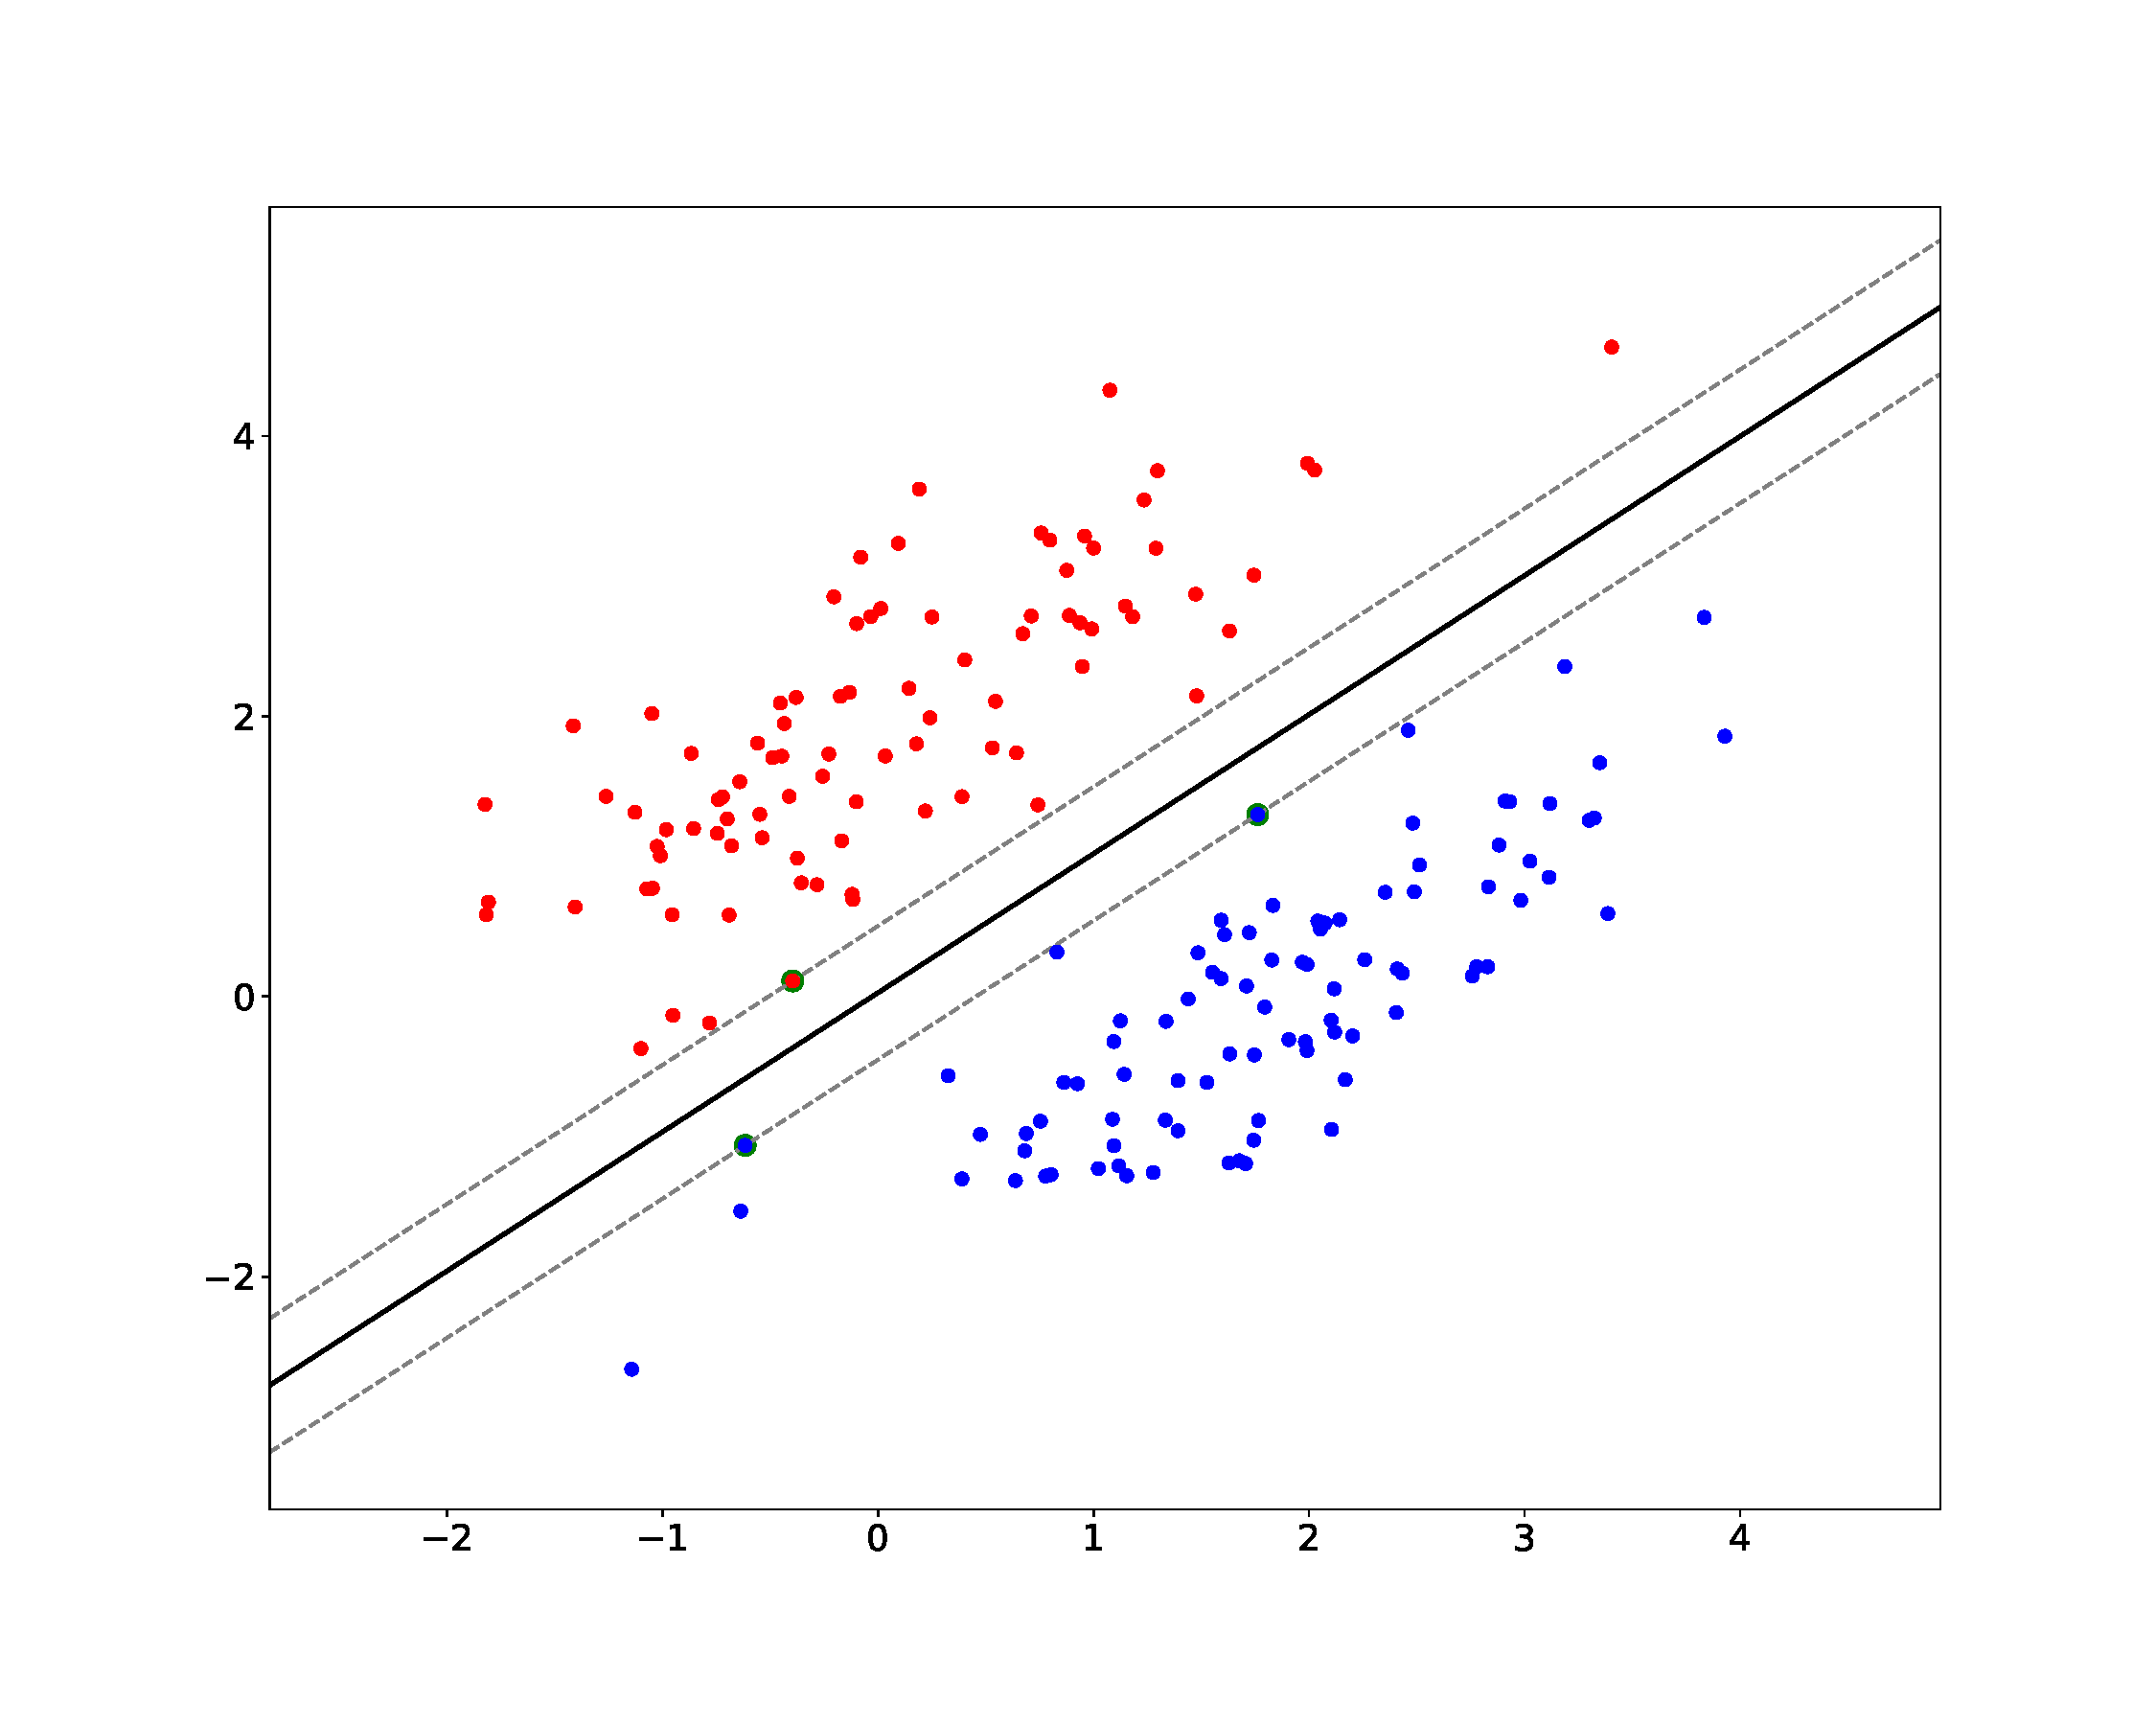
\includegraphics[scale=0.2]{11_svm/02_img/svm_linear}
	\end{figure}
\end{frame}


% Section: Non-linear / Kernel SVMs
%______________________________________________________________________
\section{Non-linear / Kernel SVMs}
\makedivider{Non-linear / Kernel SVMs}

% Non-Linear SVMs
\begin{frame}{Non-Linear SVMs / Non-Linear Separability}{}
	\divideTwo{0.49}{
		\begin{itemize}
			\item So far we have assumed \textbf{linear separability} of the data
			\item \textbf{What if the data is not linearly separable?} \\
				{\footnotesize(which will be the case in practice...)}
			\item We cannot find a straight line...
			\item $\overset{Remedy}{\Longrightarrow}$ \highlight{Feature maps}, \highlight{Kernels}
		\end{itemize}
	}{0.49}{
		\begin{figure}
			\centering
			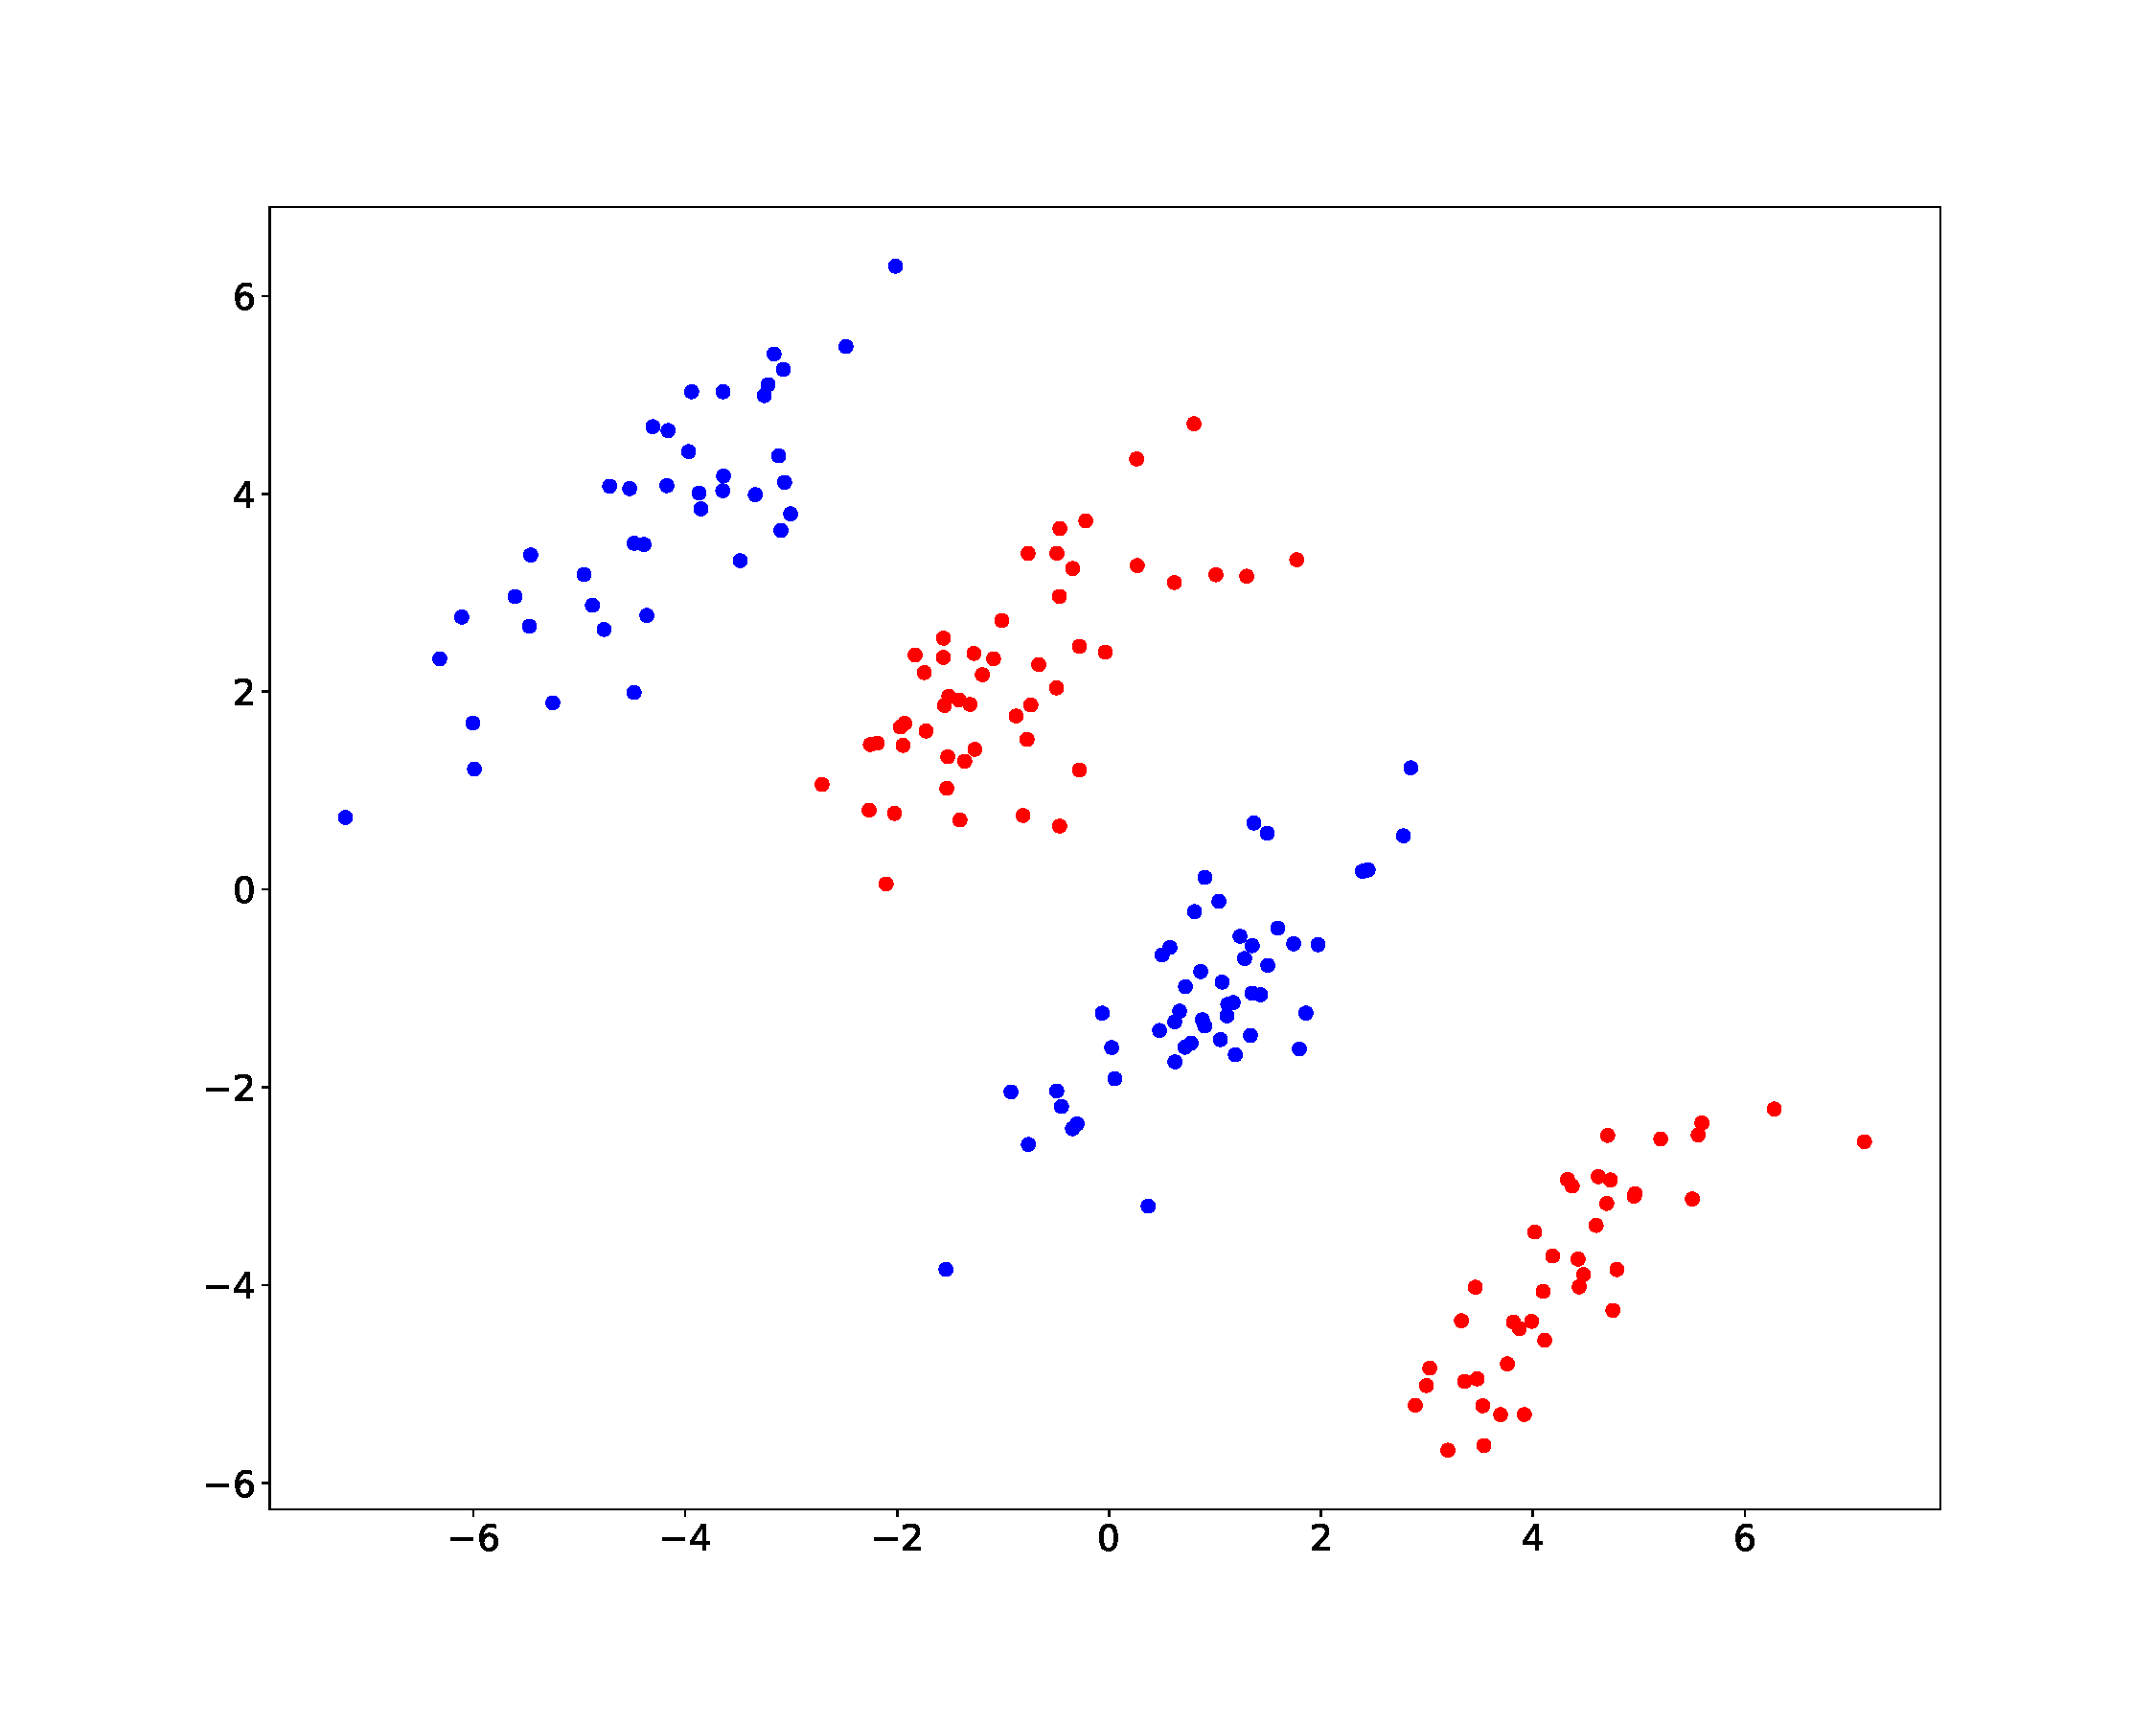
\includegraphics[scale=0.18]{11_svm/02_img/data_non_linear}
		\end{figure}
	}
\end{frame}


% Subsection: Feature Mapping
% --------------------------------------------------------------------------------------------------------
\subsection{Feature Mapping}

% Feature Mapping
\begin{frame}{Feature Mapping}{}
	The mapping function $\varphi$ maps from input space $\mathcal{X}$ to feature space $\mathcal{F}$:
	\begin{figure}
		\centering
		\begin{figure}
	\centering
	\begin{tikzpicture}[
		scale=0.6
	]
		
		\node[align=center] at (-10,0) {$\mathcal{X}$ \\ \tiny Input space};
		\node (X) at (-5,0) {
			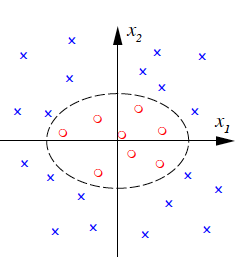
\includegraphics[scale=0.5]{11_svm/02_img/input_space}
		};

		\node[align=center] at (10,0) {$\mathcal{F}$ \\ \tiny Feature space};
		\node (F) at (5,0) {
			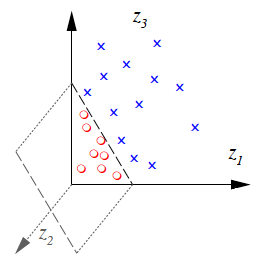
\includegraphics[scale=0.5]{11_svm/02_img/feature_space}
		};

		\draw[->,ultra thick] (X) -- node[above] {$\varphi : \mathcal{X} \mapsto \mathcal{F}$} (F);
		
	\end{tikzpicture}
\end{figure}
	\end{figure}
	\vspace*{-2mm}
	\begin{equation*}
		\varphi(x_1, x_2) \mapsto \left( x_1^2, \sqrt{2} x_1 x_2, x_2^2 \right) = (z_1, z_2, z_3)
	\end{equation*}
\end{frame}


% Feature Mapping (Ctd.)
\begin{frame}{Feature Mapping (Ctd.)}{}
	\begin{itemize}
		\item A \highlight{feature map} \textbf{explicitly} transforms the data to a higher dimension where classification becomes easier
		\item Computing the feature map can -- from a computational point of view -- become very expensive
		\item And how do you know how many dimensions to add? What transformations should be used?
		\item \highlight{A more tractable solution is required $\Rightarrow$ Kernels}
	\end{itemize}
\end{frame}


% Subsection: Kernels
% --------------------------------------------------------------------------------------------------------
\subsection{Kernels}

% What is a Kernel?
\begin{frame}{What is a Kernel?}{}
	\begin{itemize}
		\item A kernel can  be considered a \textbf{similarity function}
		\item Many algorithms have been \textit{`kernelized'}, e.\,g. \textit{Kernel PCA}, \textit{Kernel SVM}
		\item Think of it as projecting the data in a higher dimensional space to make it linearly separable
	\end{itemize}
	
	\vspace*{2mm}
	\begin{boxBlueNoFrame}
		\footnotesize
		A kernel allows the SVM to operate in a \highlight{high-dimensional, implicit feature space} without ever
		computing the coordinates of the data in that space, but rather by simply computing the \textbf{inner products}
		between the images of \textbf{all pairs of data} in the feature space. $\Rightarrow$ \highlight{Kernel trick} [Wikipedia]
	\end{boxBlueNoFrame}
\end{frame}


% What is a Kernel? (Ctd.)
\begin{frame}{What is a Kernel? (Ctd.)}{}\important
	\begin{itemize}
		\item The explicit computation of a feature map $\varphi(\bm{x})$ is avoided...
		\item ...by replacing the dot product with the kernel $\mathcal{K}$:
		\begin{equation}
			\mathcal{K}(\bm{x}, \bm{x'}) \Leftrightarrow \varphi(\bm{x})^{\intercal} \varphi(\bm{x'})
		\end{equation}
		\item Instead of mapping features explicitly, we calculate the \highlight{Gram matrix}
			$\bm{K} \in \mathbb{R}^{n \times n}$, where: 
		\begin{equation}
			K_{ij} = \mathcal{K}(\bm{x}^{(i)}, \bm{x}^{(j)})
		\end{equation}
	\end{itemize}
\end{frame}


% Well-known Kernels
\begin{frame}{Well-known Kernels}{}\important
	\begin{itemize}
		\item \highlight{Linear kernel}
		\begin{equation}
			\mathcal{K}(\bm{x}, \bm{x'}) = \bm{x}^{\intercal} \bm{x'}
		\end{equation}
		\item \highlight{Polynomial kernel}
		\begin{equation}
			\mathcal{K}(\bm{x}, \bm{x'}) = (\bm{x}^{\intercal}\bm{x'} + c)^p
		\end{equation}
		\item \highlight{Radial-Basis-Function (RBF) kernel}
		\begin{equation}
			\mathcal{K}(\bm{x}, \bm{x'}) = \exp \left\{ -\frac{\Vert \bm{x} - \bm{x'} \Vert^2}{2 \sigma^2} \right\}
				= \exp \{ -\gamma \Vert \bm{x} - \bm{x'} \Vert^2 \}
		\end{equation}
	\end{itemize}
\end{frame}


% Power of Kernels
\begin{frame}{Power of Kernels}{}
	\begin{itemize}
		\item Suppose $\bm{x}, \bm{x'} \in \mathbb{R}^m$ with $m = 2$
		\item Polynomial feature mapping ($c = 0$):
		\vspace*{-1.5mm}
		\begin{equation}
			\varphi(\bm{x}) = [x_1 x_1, x_1 x_2, x_2 x_1, x_2 x_2]^{\intercal} \qquad
			\varphi(\bm{x'}) = [x'_1 x'_1, x'_1 x'_2, x'_2 x'_1, x'_2 x'_2]^{\intercal}
		\end{equation}
		\item Using a polynomial kernel:
		{\scriptsize
		\begin{equation}
			\mathcal{K}(\bm{x}, \bm{x'}) 
				= (\bm{x}^{\intercal} \bm{x'})^2
				= \left( \sum_{i=1}^m x_i x'_i \right) \left( \sum_{j=1}^m x_j x'_j \right)
				= \sum_{i=1}^m \sum_{j=1}^m (x_i x_j) (x'_i x'_j) = \varphi(\bm{x})^{\intercal} \varphi(\bm{x'})
		\end{equation}}
	\end{itemize}
	
	\vspace*{-3mm}
	\begin{boxBlueNoFrame}
		\footnotesize
		\highlight{We need $\mathcal{O}(n^2)$ to compute $\varphi(\bm{x})$ and $\varphi(\bm{x'})$, but $\mathcal{O}(n)$
		to compute $\mathcal{K}(\bm{x}, \bm{x'})$}
	\end{boxBlueNoFrame}
\end{frame}


% Incorporating the Kernel Function
\begin{frame}{Incorporating the Kernel Function}{}
	\begin{itemize}
		\item The kernel function $\mathcal{K}$ replaces each occurrence of $\bm{x}^{\intercal}\bm{x'}$
		\item \textbf{Example:}
		\begin{align}
			\widetilde{\mathcal{L}} 
					&= \sum_{i=1}^n \alpha_i  - \frac{1}{2} \sum_{i=1}^n \sum_{j=1}^n
						\alpha_i \alpha_j y^{(i)} y^{(j)} \mathcal{K}(\bm{x}^{(i)}, \bm{x}^{(j)}) \\[4mm]
			h(\bm{x}) 	&= sign\left( \sum_{i \in \mathcal{S}} \alpha_i y^{(i)} \mathcal{K}(\bm{x}^{(i)}, \bm{x}) + b \right)
		\end{align}
	\end{itemize}
\end{frame}


% Polynomial Kernel vs. RBF Kernel
\begin{frame}{Polynomial Kernel vs. RBF Kernel}{}
	\divideTwo{0.49}{
		\begin{figure}
			\centering
			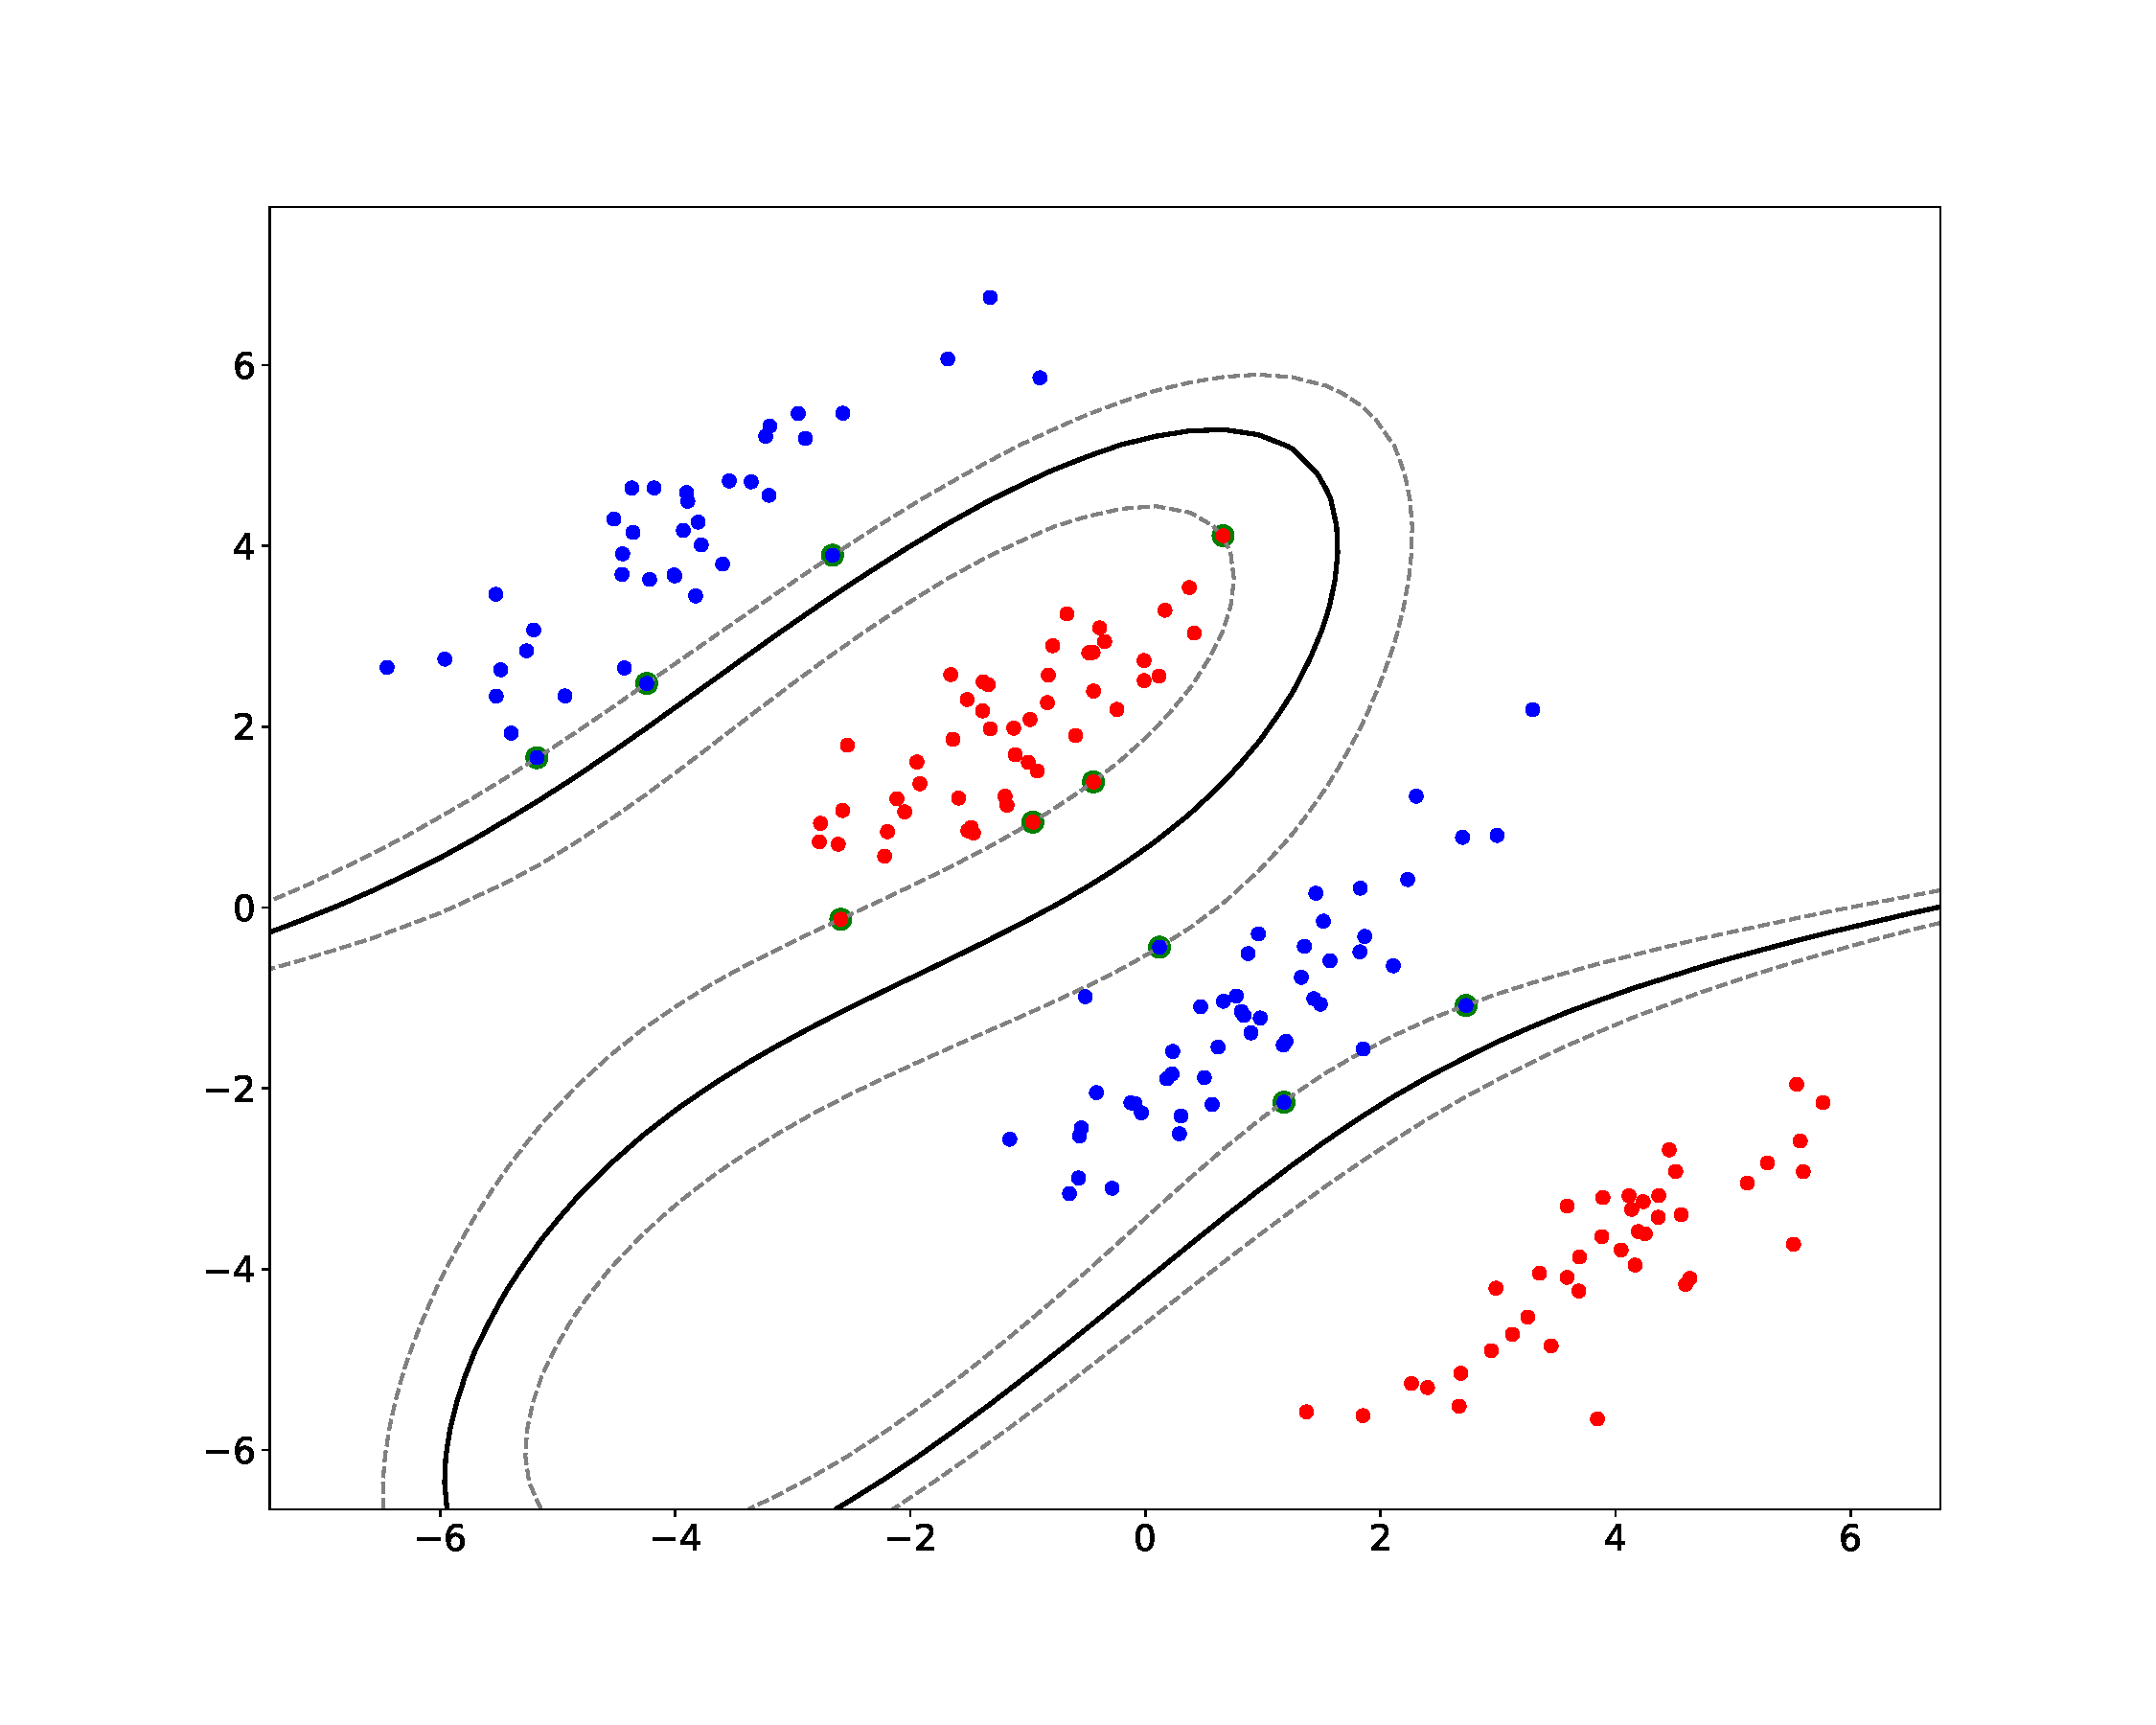
\includegraphics[scale=0.2]{11_svm/02_img/poly_kernel}
			\caption{Polynomial Kernel}
		\end{figure}
	}{0.49}{
		\begin{figure}
			\centering
			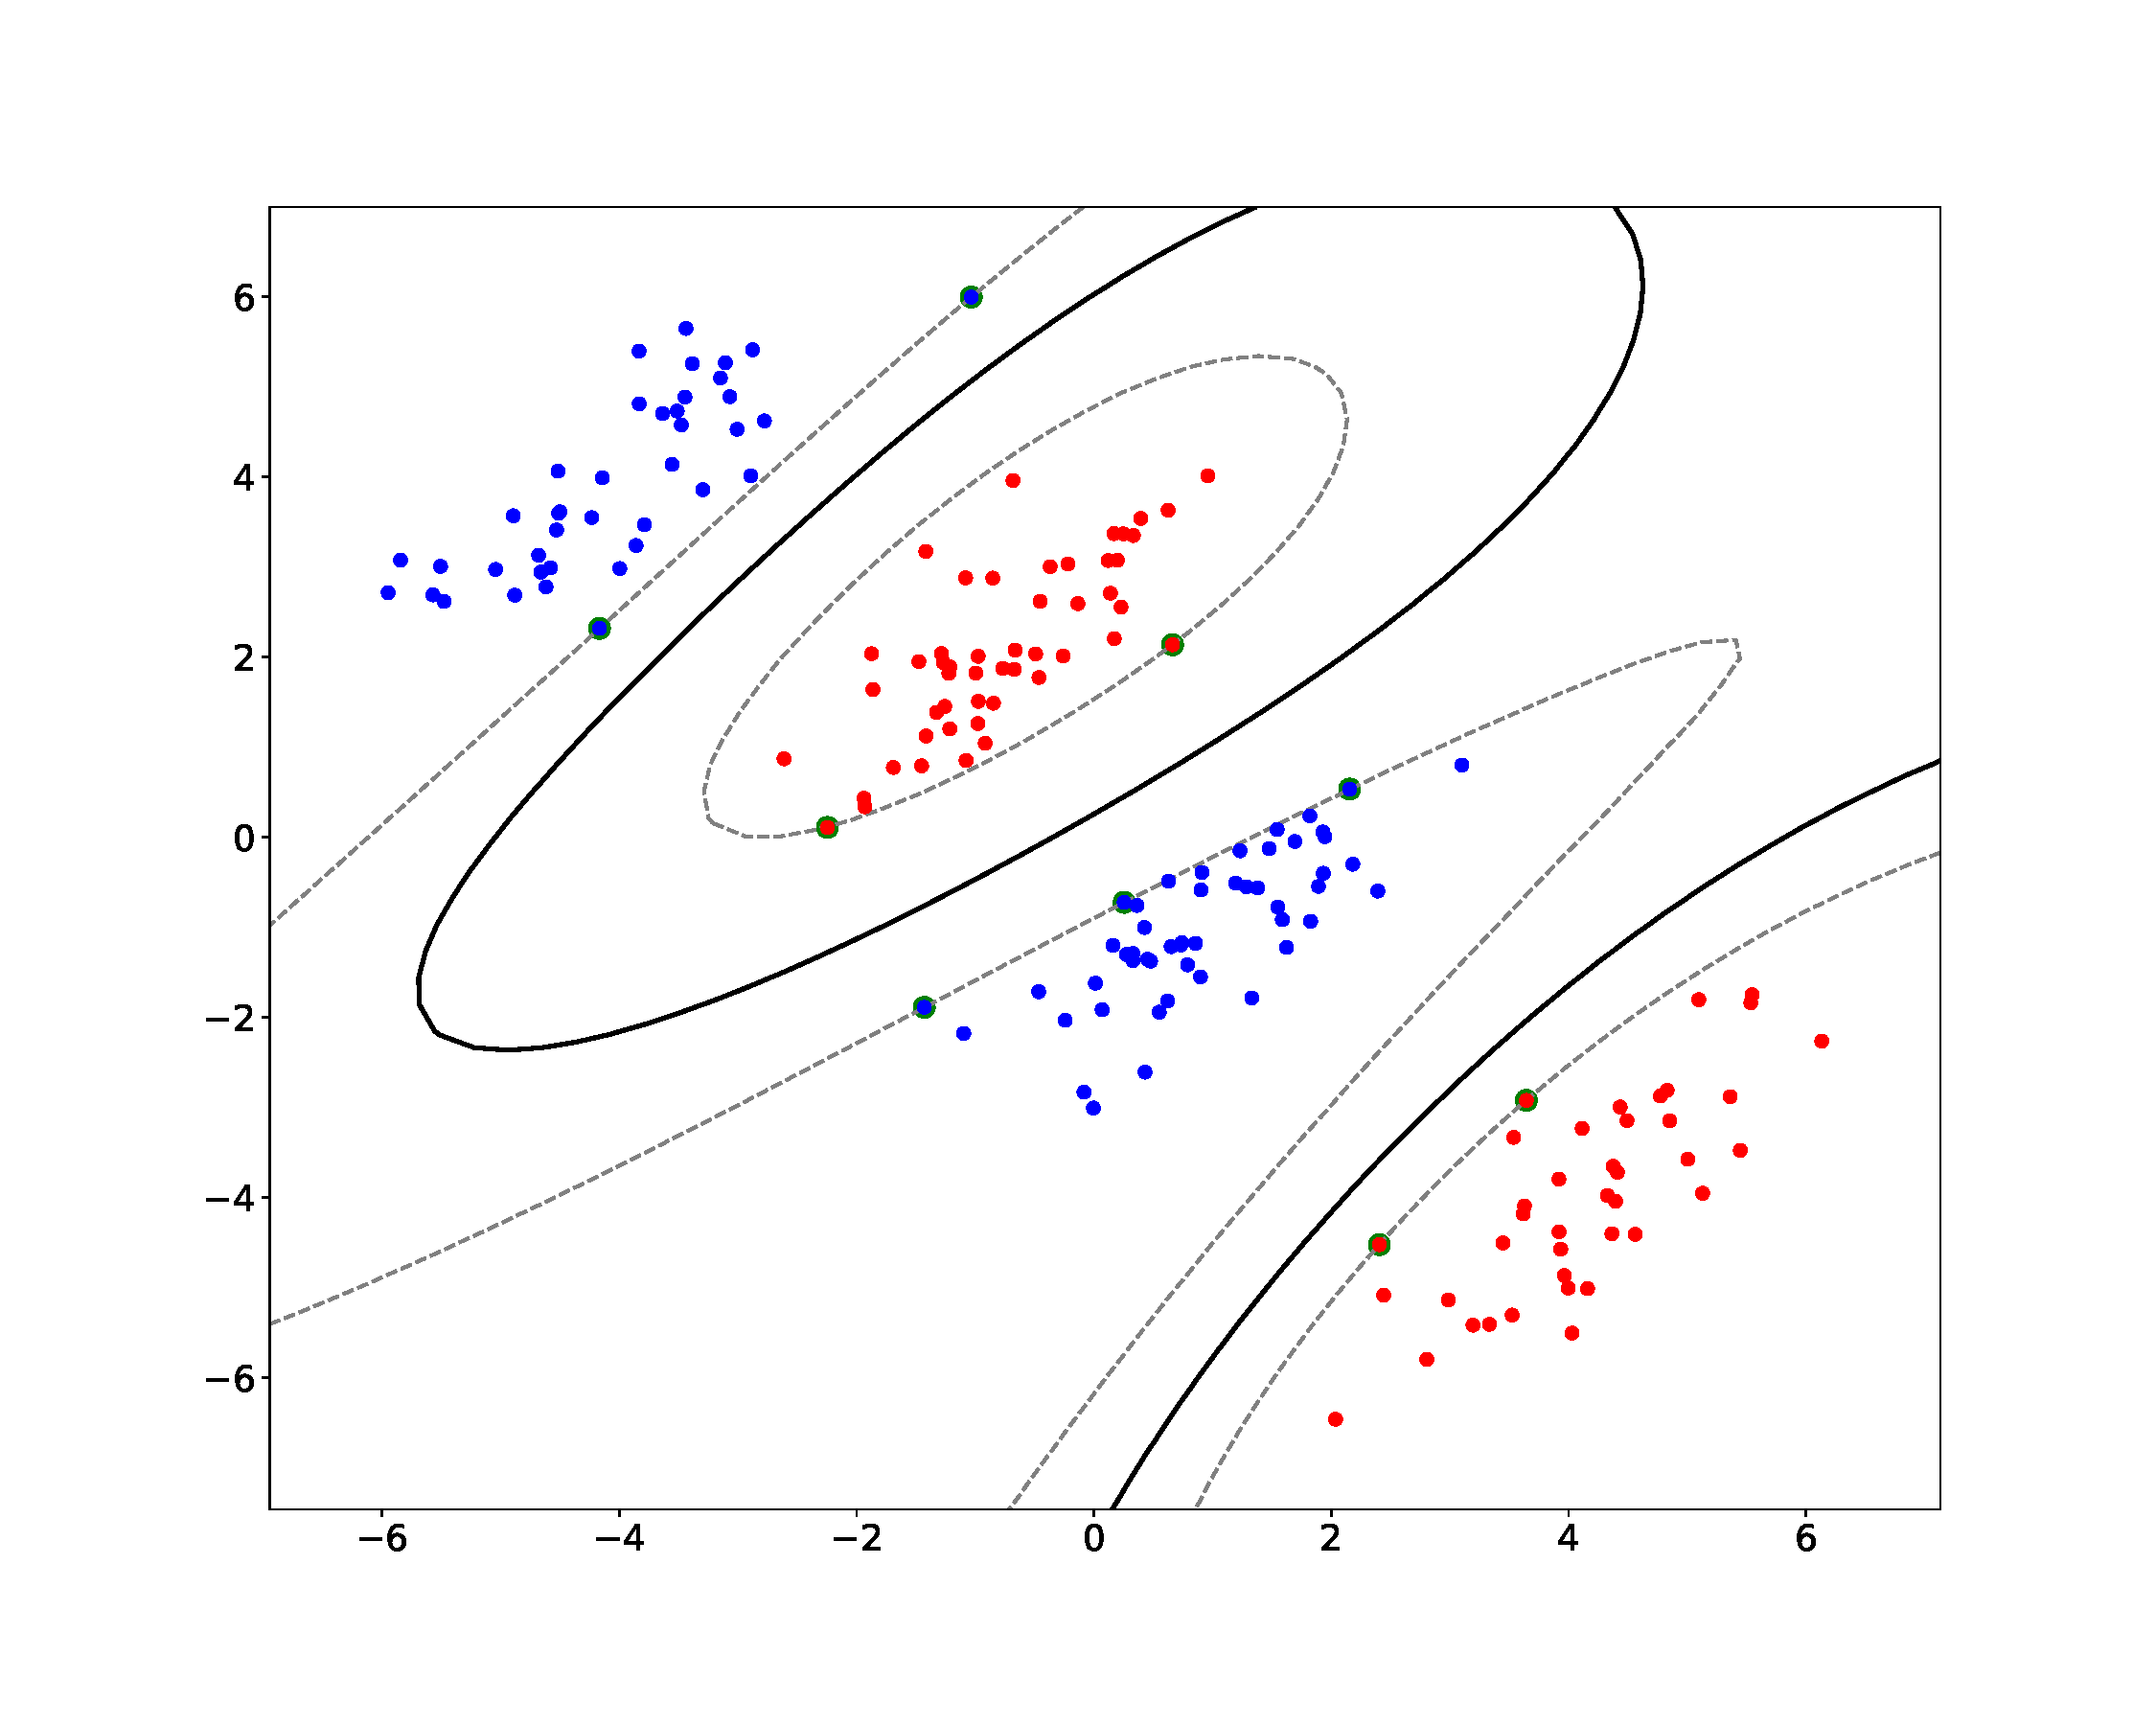
\includegraphics[scale=0.2]{11_svm/02_img/rbf_kernel}
			\caption{RBF (Gaussian) Kernel}
		\end{figure}
	}
\end{frame}


% Subsection: Mercer's Condition
% --------------------------------------------------------------------------------------------------------
\subsection{Mercer's Condition}

% Mercer's Condition
\begin{frame}{Mercer's Condition}{}
	\begin{itemize}
		\item A kernel is valid, if it fulfills \highlight{Mercer's condition}
		\item This is the case, if for all \textbf{square-integrable functions} $g(\bm{x})$...
		\begin{equation}
			\int_{-\infty}^{\infty} \vert g(\bm{x}) \vert^2 \diff \bm{x} < \infty
		\end{equation}
		\item ...it holds:
		\begin{equation}
			\int \int g(\bm{x})\mathcal{K}(\bm{x}, \bm{x'})g(\bm{x'}) \diff \bm{x} \diff \bm{x'} \ge 0
		\end{equation}
	\end{itemize}
\end{frame}


% Mercer's Condition (Ctd.)
\begin{frame}{Mercer's Condition (Ctd.)}{}\optional
	\begin{itemize}
		\item Suppose $\mathcal{K}$ is a valid kernel and let $\bm{X} = \{\bm{x}^{(1)}, \dots, \bm{x}^{(n)}\}$ be given
		\item For any vector $\bm{z} \in \mathbb{R}^n$:
		\vspace*{-1.5mm}
		\scriptsize
		\begin{align}
			\bm{z}^{\intercal} \bm{K} \bm{z}
				&= 	\sum_i \sum_j z_i K_{ij} z_j
						= \sum_i \sum_j z_i \varphi(\bm{x}^{(i)})^{\intercal} \varphi(\bm{x}^{(j)}) z_j 			\\
				&= \sum_i \sum_j z_i \sum_k (\varphi(\bm{x}^{(i)}))_k (\varphi(\bm{x}^{(j)}))_k z_j 
						= \sum_k \sum_i \sum_j z_i (\varphi(\bm{x}^{(i)}))_k (\varphi(\bm{x}^{(j)}))_k z_j 		\\
				&= \sum_k \left( \sum_i z_i \varphi(\bm{x}^{(i)})_k \right)^2 \ge 0 \Longrightarrow \bm{K} \ge 0
		\end{align}
		\normalsize
		\item $\bm{K} \ge 0$ means that matrix $\bm{K}$ must be \highlight{positive semi-definite (psd)}
	\end{itemize}
\end{frame}


% Mercer's Condition (Ctd.)
\begin{frame}{Mercer's Condition (Ctd.)}{}\important
	\begin{boxBlue}
		\highlight{Mercer's Theorem:} \\
		$\mathcal{K}$ is a valid kernel, iff for any set of $n$ training examples $\bm{X} = \{ \bm{x}^{(1)}, \dots, \bm{x}^{(n)} \}$ kernel matrix
		$\bm{K} \in \mathbb{R}^{n \times n}$ is \textbf{positive semi-definite}. The kernel is then called \highlight{Mercer kernel}.
	\end{boxBlue}

	\begin{itemize}
		\item This entails: $K_{ij} \ge 0\ \forall i, j$
		\item \textbf{Example}:
		\begin{itemize}
			\item $\mathcal{K}(\bm{x}, \bm{x}) = -1 \ne \varphi(\bm{x})^{\intercal} \varphi(\bm{x})$
			\item $\mathcal{K}$ cannot be a valid kernel
		\end{itemize}
	\end{itemize}
\end{frame}


% Constructing new Kernels
\begin{frame}{Constructing new Kernels}{}
	\begin{itemize}
		\item It is not always easy to check if Mercer's condition is satisfied, but it is possible to construct
			\textbf{new kernels out of known ones}
		\item If $\mathcal{K}_1(\bm{x}, \bm{x'})$ and $\mathcal{K}_2(\bm{x}, \bm{x'})$ are valid kernels, so are:
	\end{itemize}
	
	\vspace*{2mm}
	\begin{boxBlueNoFrame}
		\begin{itemize}
			\setlength\itemsep{0em}
			\item $c \cdot \mathcal{K}_1(\bm{x}, \bm{x'})$
			\item $\mathcal{K}_1(\bm{x}, \bm{x'}) + \mathcal{K}_2(\bm{x}, \bm{x'})$
			\item $\mathcal{K}_1(\bm{x}, \bm{x'}) \cdot \mathcal{K}_2(\bm{x}, \bm{x'})$
			\item $f(\bm{x}) \cdot \mathcal{K}_1(\bm{x}, \bm{x'}) \cdot f(\bm{x'})$
			\item etc.
		\end{itemize}
	\end{boxBlueNoFrame}
\end{frame}


% Section: Soft-Margin SVMs
%______________________________________________________________________
\section{Soft-Margin SVMs}
\makedivider{Soft-Margin SVMs}

% Subsection: Overlapping Data
% --------------------------------------------------------------------------------------------------------
\subsection{Overlapping Data}

% Overlapping Distributions
\begin{frame}{Overlapping Distributions}{}
	\begin{itemize}
		\item We assumed linearly separable data \\
			\hspace*{5mm} $\Rightarrow$ \textbf{SVM gives exact solution}
		\item \textbf{But:} The classes may overlap \\
			\hspace*{5mm} $\Rightarrow$ \textbf{Exact separation leads to poor generalization}
		\item \highlight{Soft-margin SVM:} Allow some data points to be misclassified
		\item To this end, a penalty is introduced:
		\begin{itemize}
			\item Misclassifications are penalized
			\item This penalty increases linearly with the distance from the decision boundary
		\end{itemize}
		\item This is done using \highlight{slack variables}
	\end{itemize}
\end{frame}


% Overlapping Distributions: Example
\begin{frame}{Overlapping Distributions: Example}{}
	\vspace*{-2mm}
	\begin{figure}
		\centering
		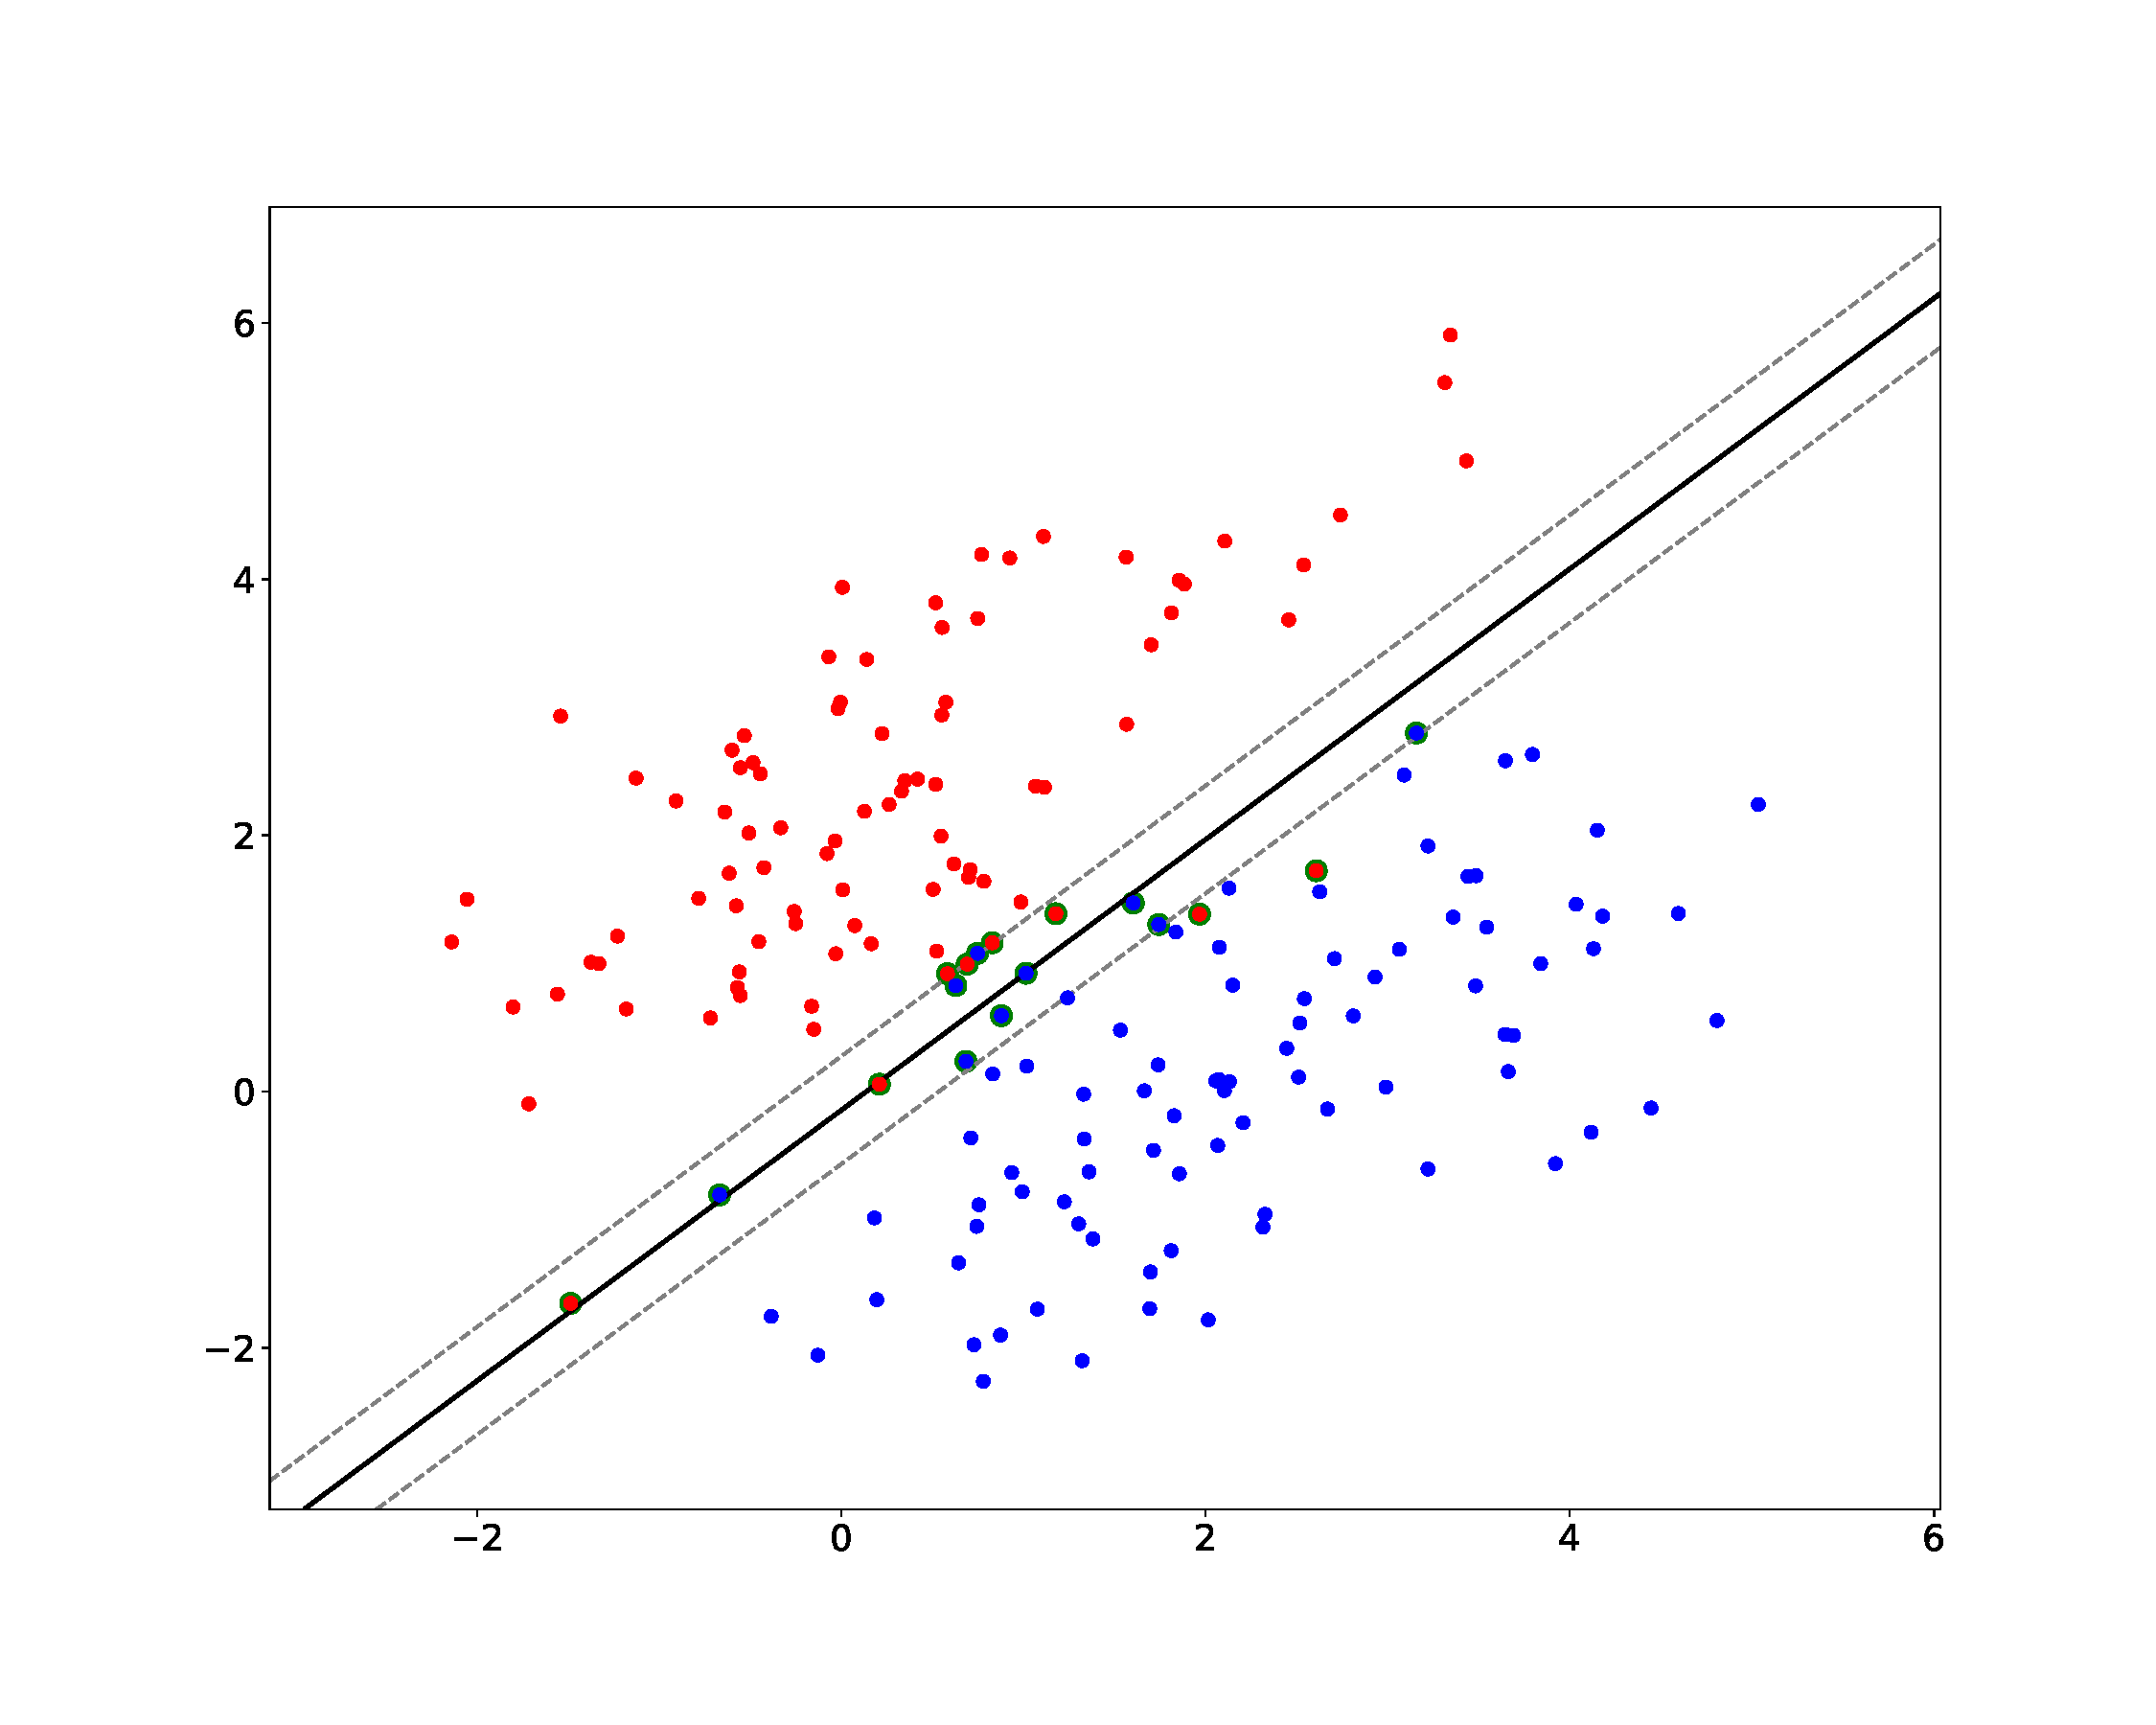
\includegraphics[scale=0.2]{11_svm/02_img/soft_margin}
	\end{figure}
\end{frame}


% Subsection: Slack Variables
% --------------------------------------------------------------------------------------------------------
\subsection{Slack Variables}

% Slack Variables
\begin{frame}{Slack Variables}{}
	\begin{itemize}
		\item The slack is denoted by $\xi_i$ (where $\xi_i \ge 0; i = 1, \dots, n$), one per data point
		\item \textbf{Different cases}:
		
		\footnotesize
		\begin{tabbing}
			\hspace*{2.5cm}\= \kill
			$\xi_i = 0$ 		\> if $\bm{x}^{(i)}$ is on or inside the correct margin boundary 		\\
			$0 < \xi_i < 1$ 		\> if $\bm{x}^{(i)}$ lies inside the margin, but on the correct side 		\\
			$\xi_i = 1$ 		\> if $\bm{x}^{(i)}$ is on the decision boundary 					\\
			$\xi_i > 1$ 		\> if $\bm{x}^{(i)}$ lies on the wrong side of the decision boundary (misclassification)
		\end{tabbing}
		\normalsize

		\item The classification constraints are replaced with:
		\begin{equation}
			y^{(i)} \widehat{h}(\bm{x}^{(i)}) \ge 1 - \xi_i \qquad i = 1, \dots, n
		\end{equation}
		\item We get a \highlight{soft-margin classifier}
	\end{itemize}
\end{frame}


% Slack Variables (Ctd.)
\begin{frame}{Slack Variables (Ctd.)}{}
	\begin{figure}
	\centering
	\begin{tikzpicture}[
		scale=0.8
	]

		\draw[thick,gray] (-0.5,0) -- (6,6.5) node[right] {y = -1};
		\draw[very thick,black] (1.25,0) -- (6,4.75) node[right] {y = 0; Decision Boundary};
		\draw[thick,gray] (3,0) -- (6,3) node[right] {y = 1};

		\draw[dashed,gray] (-4,6.5) -- ++(3,0) -- (5,5.5); \node[fill=white] at (-4,6.5) {\scriptsize $\xi_1 > 1$};
		\draw[dashed,gray] (-4,6) -- ++(3,0) -- (4,4); \node[fill=white] at (-4,6) {\scriptsize $\xi_2 > 1$};
		\draw[dashed,gray] (-4,5.5) -- ++(3,0) -- (4,2.75); \node[fill=white] at (-4,5.5) {\scriptsize $\xi_3 = 1$};
		\draw[dashed,gray] (-4,5) -- ++(3,0) -- (4.5,1.5); \node[fill=white] at (-4,5) {\scriptsize $\xi_4 = 0$};
		\draw[dashed,gray] (-4,4.5) -- ++(3,0) -- (4.25,0.75); \node[fill=white] at (-4,4.5) {\scriptsize $\xi_5 = 0$};
		\draw[dashed,gray] (-4,4) -- ++(3,0) -- (2.5,0.5); \node[fill=white] at (-4,4) {\scriptsize $\xi_6 < 1$};
		
		\doublecircle{5}{5.5}
		\doublecircle{4}{2.75}
		\doublecircle{4.5}{1.5}
		\doublecircle{4}{4}
		\doublecircle{2.5}{0.5}
		\doublecircle{4.25}{0.75}

		\draw (-4.75,3.75) rectangle (-3.25,6.75);

		\node[myblue1] at (7,1.25) {\textbf{Class +1}};
		
	\end{tikzpicture}
\end{figure}
\end{frame}


% Soft SVM Parameter Optimization
\begin{frame}{Soft SVM Parameter Optimization}{}
	\begin{itemize}
		\item We want to maximize the margin, while softly \textbf{penalizing points which lie on the wrong side of the boundary}:
		\begin{equation}
			\frac{1}{2} \Vert \bm{w} \Vert^2 + C \sum_{i=1}^n \xi_i
			\quad \text{s.\,t.} \quad y^{(i)} \widehat{h}(\bm{x}^{(i)}) \ge 1 - \xi_i\ \text{and}\ \xi_i \ge 0\ \forall i
		\end{equation}
		\item $C > 0$ controls the \textit{`degree of softness'}, the larger $C$ the more we penalize
		\item The Lagrangian function:
		
		\footnotesize
		\vspace*{-2mm}
		\begin{equation}
			\mathcal{L}(\bm{w}, b, \bm{\alpha}, \bm{\mu})
				= \frac{1}{2} \Vert \bm{w} \Vert^2 + C \sum_{i=1}^n \xi_i -
					\sum_{i=1}^n \alpha_i \{ y^{(i)} \widehat{h}(\bm{x}^{(i)}) - 1 + \xi_i \} - \sum_{i=1}^n \mu_i \xi_i
		\end{equation}
	\end{itemize}
\end{frame}


% Soft SVM Parameter Optimization (Ctd.)
\begin{frame}{Soft SVM Parameter Optimization (Ctd.)}{}
	\begin{itemize}
		\item It turns out that the dual objective function looks exactly the same:
		\begin{equation}
			\widetilde{\mathcal{L}}(\bm{\alpha}) =
				\sum_{i=1}^n \alpha_i - \frac{1}{2} \sum_{i=1}^n \sum_{j=1}^n
				\alpha_i \alpha_j y^{(i)} y^{(j)} \langle \bm{x}^{(i)}, \bm{x}^{(j)} \rangle
		\end{equation}
		\item But the constraints differ slightly:
		\footnotesize
		\begin{align}
			&1) \quad \sum_{i=1}^n \alpha_i y^{(i)} = 0 \\[2mm]
			&2) \quad \boxed{0 \le \alpha_i\ \textcolor{red}{\le C} \qquad i = 1, \dots, n} 
		\end{align}
		\normalsize
		\item Constraint 2) is called \highlight{boxed constraint}
	\end{itemize}
\end{frame}


% Section: Multi-Class Classification
%______________________________________________________________________
\section{Multi-Class Classification}
\makedivider{Multi-Class Classification}

% Subsection: Multiple Classes
% --------------------------------------------------------------------------------------------------------
\subsection{Multiple Classes}

% Multi-Class Classification
\begin{frame}{Multi-Class Classification}{}
	\begin{itemize}
		\item An SVM can handle two classes only, namely \textbf{-1} and \textbf{+1}
		\item \textbf{What if there are more than two classes?}
		\item Two common techniques:
		\begin{itemize}
			\item \highlight{One-vs-Rest (OVR)} 	$\Rightarrow$ One-against-All
			\item \highlight{One-vs-One (OVO)} 	$\Rightarrow$ Pairwise classification
		\end{itemize}
		\item Several classifiers are trained
		\item During prediction the classifiers \textbf{vote for the correct class}
		\item Such techniques can be used for all binary classifiers (e.\,g. logistic regression)
	\end{itemize}
\end{frame}


% Subsection: One-vs-Rest (OVR)
% --------------------------------------------------------------------------------------------------------
\subsection{One-vs-Rest (OVR)}

% Multi-Class Classification: One-vs-Rest (OVR)
\begin{frame}{Multi-Class Classification: One-vs-Rest (OVR)}{}
	\divideTwo{0.49}{
		\begin{itemize}
			\item \textbf{Train one classifier per class} (expert for that class)
			\item We get $\vert \mathcal{C} \vert$ classifiers
			\item The $k$-th classifier learns to distinguish the $k$-th class from all the others
			\item Set the labels of examples from class $k$ to \textbf{+1}, all the others to \textbf{-1}
		\end{itemize}
	}{0.49}{
		\vspace*{2mm}
		\begin{figure}
	\centering
	\begin{tikzpicture}[
		scale=0.8
	]

		\begin{axis}[
			xlabel={$x_1$},
			ylabel={$x_2$}
		]
		
			\addplot[
				only marks,mark=*,mark size=2.0,fill=red,discard if not={c}{0}
			] table{11_svm/05_data/data_multi_class.txt};

			\addplot[
				only marks,mark=*,mark size=2.0,fill=blue,discard if not={c}{1}
			] table{11_svm/05_data/data_multi_class.txt};

			\addplot[
				only marks,mark=*,mark size=2.0,fill=green,discard if not={c}{2}
			] table{11_svm/05_data/data_multi_class.txt};

			\draw[thick,dashed,red] (axis cs: -15,-24) -- (axis cs: -3,0) -- (axis cs: -15,30);
			\node[red] at (axis cs: -10,-6) {\textbf{+1}};
			\node at (axis cs: 0,0) {\textbf{-1}};
			
    		\end{axis}
		
	\end{tikzpicture}
\end{figure}
	}
\end{frame}


% Subsection: One-vs-One (OVO)
% --------------------------------------------------------------------------------------------------------
\subsection{One-vs-One (OVO)}

% Multi-Class Classification: One-vs-One (OVO)
\begin{frame}{Multi-Class Classification: One-vs-One (OVO)}{}
	\divideTwo{0.49}{
		\vspace*{2mm}
		\begin{figure}
	\centering
	\begin{tikzpicture}[
		scale=0.8
	]

		\begin{axis}[
			xlabel={$x_1$},
			ylabel={$x_2$}
		]
		
			\addplot[
				only marks,mark=*,mark size=2.0,fill=red,discard if not={c}{0}
			] table{11_svm/05_data/data_multi_class.txt};

			\addplot[
				only marks,mark=*,mark size=2.0,fill=blue,discard if not={c}{1}
			] table{11_svm/05_data/data_multi_class.txt};

			\addplot[
				only marks,mark=*,mark size=2.0,fill=white,draw=gray,discard if not={c}{2}
			] table{11_svm/05_data/data_multi_class.txt};

			\draw[thick,dashed,red] (axis cs: -10,-10) -- (axis cs: 5,7.5);
			\node[red] at (axis cs: -10,-6) {\textbf{+1}};
			\node[blue] at (axis cs: -5,-7.5) {\textbf{-1}};
			\node[gray] at (axis cs: -2.5,7.5) {ignored};
			
    		\end{axis}
		
	\end{tikzpicture}
\end{figure}
	}{0.49}{
		\begin{itemize}
			\item \textbf{Train one classifier for each pair of classes}
			\item We get $\binom{\vert \mathcal{C} \vert}{2}$ classifiers
			\item Ignore all other examples that do not belong to either of the two classes
			\item \textbf{Voting}: Count how often each class wins; the class with the highest score is predicted
		\end{itemize}
	}
\end{frame}


% Section: Wrap-Up
%______________________________________________________________________
\section{Wrap-Up}
\makedivider{Wrap-Up}

% Subsection: Summary
% --------------------------------------------------------------------------------------------------------
\subsection{Summary}

% Summary
\begin{frame}{Summary}{}
	\begin{itemize}
		\item SVMs  assume the data to be \textbf{linearly separable}
		\item \textbf{Generalization guarantee:} SVMs are \textbf{maximum margin} classifiers
		\item The set of \textbf{support vectors} defines the decision boundary
		\item We have to solve a quadratic optimization problem to obtain the support vectors which are needed for prediction
		\item \Highlight{Important concept:} Kernels (cf. Mercer's condition)
		\item Slack variables allow for \textbf{soft-margin classification}
		\item Apply multi-class classification techniques like OVR / OVO if you have more than two classes
	\end{itemize}
\end{frame}


% Subsection: Self-Test Questions
% --------------------------------------------------------------------------------------------------------
\subsection{Self-Test Questions}

% Self-Test Questions
\begin{frame}{Self-Test Questions}{}\important
	\begin{enumerate}
		\item What is a maximum-margin classifier?
		\item Which data points are needed for prediction? How do we get them?
		\item What is a kernel? Can every function serve as a kernel?
		\item What prerequisite allows for the usage of kernels?
		\item Name famous kernels and write down the equation to compute them!
		\item What is slack? What can we do with it?
	\end{enumerate}
\end{frame}


% Subsection: Lecture Outlook
% --------------------------------------------------------------------------------------------------------
\subsection{Lecture Outlook}

\begin{frame}{What's next...?}{}
	\makeoverview{9}
\end{frame}


% Subsection: Recommended Literature and further Reading
% --------------------------------------------------------------------------------------------------------
\subsection{Recommended Literature and further Reading}

% Literature
%______________________________________________________________________
\begin{frame}[allowframebreaks]{Recommended Literature and further Reading}{}
	\footnotesize
	\begin{thebibliography}{2}
		\literature{book}{Bishop.2006}{[1] Pattern Recognition and Machine Learning}
			{Christopher Bishop. Springer. 2006.}{$\rightarrow$ \href{
				http://users.isr.ist.utl.pt/~wurmd/Livros/school/Bishop\%20-\%20Pattern\%20Recognition\%20And\%20Machine\%20Learning\%20-\%20Springer\%20\%202006.pdf
			}{\linkstyle{Link}}, cf. chapter 7}
			
		\literature{book}{Murphy.2012}{[2] Machine Learning: A Probabilistic Perspective}
			{Kevin Murphy. MIT Press. 2012.}{$\rightarrow$ \href{
				https://doc.lagout.org/science/Artificial\%20Intelligence/Machine\%20learning/Machine\%20Learning_\%20A\%20Probabilistic\%20Perspective\%20\%5BMurphy\%202012-08-24\%5D.pdf
			}{\linkstyle{Link}}, cf. chapter 14.5}
	\end{thebibliography}
\end{frame}


% Subsection: Meme of the Day
% --------------------------------------------------------------------------------------------------------
\subsection{Meme of the Day}

% Meme of the Day
\begin{frame}{Meme of the Day}{}
	\begin{figure}
		
\includegraphics[scale=0.8]{11_svm/02_img/meme_of_the_day}
	\end{figure}
\end{frame}


% Thank you
%______________________________________________________________________
\makethanks

\end{document}